% =============================================================================
%  Diplomado en Data Science Aplicada con Python para la Toma de Decisiones
%  Clase 24: CNN --- De MLP a Convoluciones (procesar imagenes en serio)
%  Arca Continental Ecuador | UDLA
%
%  Compilar: pdflatex -shell-escape presentacion.tex (x2 para refs)
% =============================================================================
\documentclass[aspectratio=169, 11pt]{beamer}

\usepackage[T1]{fontenc}
\usepackage[utf8]{inputenc}
\usepackage[spanish,es-noshorthands]{babel}
\usepackage{FiraSans}
\usepackage{FiraMono}
\renewcommand{\familydefault}{\sfdefault}
\usepackage{graphicx}
\usepackage{tikz}
\usetikzlibrary{arrows.meta, positioning, shapes.geometric, shapes.misc,
  calc, fit, decorations.pathreplacing, backgrounds}
\usepackage{fontawesome5}
\usepackage{minted}
\usepackage{tcolorbox}
\tcbuselibrary{minted, skins, breakable}
\usepackage{booktabs}
\usepackage{colortbl}
\usepackage{multicol}
\usepackage{hyperref}
\usepackage{calc}
\usepackage{amsmath}

\definecolor{arcaRed}{HTML}{C82B40}
\definecolor{arcaDark}{HTML}{6B1525}
\definecolor{udlaCrimson}{HTML}{A31545}
\definecolor{arcaGray}{HTML}{F5F5F5}
\definecolor{arcaLightGray}{HTML}{EBEBEB}
\definecolor{textDark}{HTML}{2D2D2D}
\definecolor{textMuted}{HTML}{6B7280}
\definecolor{codeGreen}{HTML}{16A34A}
\definecolor{codeBlue}{HTML}{2563EB}
\definecolor{codeOrange}{HTML}{EA580C}
\definecolor{codePurple}{HTML}{7C3AED}

\usetheme{default}
\usecolortheme{default}
\setbeamertemplate{navigation symbols}{}
\setbeamertemplate{footline}{}
\setbeamertemplate{headline}{}
\setbeamercolor{normal text}{fg=textDark}
\setbeamercolor{frametitle}{fg=arcaRed, bg=white}
\setbeamercolor{title}{fg=white}
\setbeamercolor{subtitle}{fg=white!85}
\setbeamercolor{author}{fg=white!80}
\setbeamercolor{date}{fg=white!70}
\setbeamercolor{item}{fg=arcaRed}
\setbeamercolor{subitem}{fg=arcaDark}
\setbeamercolor{block title}{fg=white, bg=arcaRed}
\setbeamercolor{block body}{fg=textDark, bg=arcaGray}
\setbeamercolor{section in toc}{fg=arcaDark}
\setbeamerfont{frametitle}{size=\Large, series=\bfseries}
\setbeamerfont{title}{size=\huge, series=\bfseries}
\setbeamerfont{subtitle}{size=\large}
\setbeamerfont{author}{size=\normalsize}
\setbeamerfont{date}{size=\small}
\setbeamerfont{block title}{size=\normalsize, series=\bfseries}
\setbeamerfont{footnote}{size=\tiny}
\setbeamertemplate{itemize item}{\scriptsize\raise1.5pt\hbox{\color{arcaRed}$\blacktriangleright$}}
\setbeamertemplate{itemize subitem}{\scriptsize\raise1pt\hbox{\color{arcaDark}$\bullet$}}
\setbeamertemplate{enumerate items}[default]
\setbeamercolor{enumerate item}{fg=arcaRed}

\setbeamertemplate{headline}{%
  \begin{tikzpicture}[remember picture, overlay]
    \fill[arcaDark] (current page.north west) rectangle
      ([yshift=-0.7cm]current page.north east);
    \node[anchor=west, inner sep=0pt] at
      ([xshift=0.6cm, yshift=-0.35cm]current page.north west)
      {
\includegraphics[height=0.45cm]{../logo_udla_white.png}};
    \node[anchor=east, inner sep=0pt] at
      ([xshift=-0.6cm, yshift=-0.35cm]current page.north east)
      {
\includegraphics[height=0.45cm]{../ArcaContinental_white.png}};
  \end{tikzpicture}%
  \vspace{0.7cm}%
}

\setbeamertemplate{footline}{%
  \begin{tikzpicture}[remember picture, overlay]
    \node[anchor=south east, font=\scriptsize\bfseries\color{arcaRed}] at
      ([xshift=-0.5cm, yshift=0.15cm]current page.south east)
      {\insertframenumber};
  \end{tikzpicture}%
  \vspace{0.3cm}%
}

\setbeamertemplate{frametitle}{%
  \vspace{0.25cm}%
  \usebeamerfont{frametitle}\usebeamercolor[fg]{frametitle}\insertframetitle%
  \par\vspace{2pt}%
  \begin{tikzpicture}
    \fill[arcaRed] (0,0) rectangle (3cm, 1.5pt);
    \fill[arcaLightGray] (3cm,0) rectangle (\textwidth, 0.5pt);
  \end{tikzpicture}%
  \vspace{0.1cm}%
}

\newtcblisting{pyblock}[1][]{%
  listing engine=minted, minted language=python, minted style=friendly,
  minted options={fontsize=\small, linenos=false, breaklines=true, python3=true},
  colback=arcaGray, colframe=arcaRed, left=4pt, right=4pt, top=4pt, bottom=4pt,
  boxrule=0pt, leftrule=3pt, arc=2pt, listing only, #1}

\newcommand{\sectionframe}[2]{%
  \begingroup
  \setbeamertemplate{headline}{}%
  \setbeamertemplate{footline}{}%
  \begin{frame}[plain, noframenumbering]
    \begin{tikzpicture}[remember picture, overlay]
      \fill[arcaRed] (current page.south west) rectangle (current page.north east);
      \node[anchor=center, text=white, font=\Huge\bfseries, text width=12cm,
            align=center] at ([yshift=0.5cm]current page.center) {#1};
      \node[anchor=center, text=white!80, font=\large, text width=10cm,
            align=center] at ([yshift=-0.8cm]current page.center) {#2};
    \end{tikzpicture}
  \end{frame}
  \endgroup
}

\title{Diplomado en Data Science Aplicada\\con Python para la Toma de Decisiones}
\subtitle{Clase 24: CNN --- Procesar Im\'agenes en Serio}
\author{Carlos Enrique Mosquera Trujillo}
\date{20 de Mayo, 2026}

\begin{document}

% ── PORTADA ──────────────────────────────────────────────────────────────────
{
\setbeamertemplate{headline}{}
\setbeamertemplate{footline}{}
\begin{frame}[plain, noframenumbering]
  \begin{tikzpicture}[remember picture, overlay]
    \fill[arcaDark] (current page.south west) rectangle (current page.north east);
    \fill[arcaRed] ([yshift=-3.5cm]current page.north west) rectangle
      ([yshift=-4.2cm]current page.north east);
    \node[anchor=west, inner sep=0pt] at
      ([xshift=1cm, yshift=-1.5cm]current page.north west)
      {
\includegraphics[height=1cm]{../logo_udla_white.png}};
    \node[anchor=east, inner sep=0pt] at
      ([xshift=-1cm, yshift=-1.5cm]current page.north east)
      {
\includegraphics[height=1cm]{../ArcaContinental_white.png}};
  \end{tikzpicture}
  \vspace{2.5cm}
  \begin{center}
    {\usebeamerfont{title}\usebeamercolor[fg]{title}\inserttitle\par}
    \vspace{0.4cm}
    {\usebeamerfont{subtitle}\usebeamercolor[fg]{subtitle}\insertsubtitle\par}
    \vspace{0.6cm}
    {\usebeamerfont{author}\usebeamercolor[fg]{author}\insertauthor\par}
    \vspace{0.15cm}
    {\usebeamerfont{date}\usebeamercolor[fg]{date}\insertdate\par}
  \end{center}
\end{frame}
}

% ── M\'ODULO 5 ─────────────────────────────────────────────────────────────────
{
\setbeamertemplate{headline}{}
\setbeamertemplate{footline}{}
\begin{frame}[plain, noframenumbering]
  \begin{tikzpicture}[remember picture, overlay]
    \fill[arcaDark] (current page.south west) rectangle (current page.north east);
    \node[anchor=center, text=white, font=\Large\bfseries, text width=12cm,
          align=center] at ([yshift=1cm]current page.center)
      {M\'odulo 5};
    \node[anchor=center, text=white!90, font=\huge\bfseries, text width=12cm,
          align=center] at ([yshift=-0.3cm]current page.center)
      {Redes Neuronales Convolucionales};
  \end{tikzpicture}
\end{frame}
}

% ── ROADMAP ─────────────────────────────────────────────────────────────────
\begin{frame}[shrink]{Hoja de Ruta}
  \vspace{4pt}
  \begin{center}
  \begin{tikzpicture}[
    node distance=0.25cm,
    roadstep/.style={rectangle, rounded corners=4pt, draw=arcaRed, fill=arcaRed!8,
                 minimum width=11cm, minimum height=0.55cm,
                 font=\footnotesize\bfseries\color{arcaDark}, align=left,
                 text width=10cm, inner sep=4pt},
    num/.style={circle, fill=arcaRed, text=white, font=\scriptsize\bfseries,
                minimum size=0.45cm, inner sep=0pt},
  ]
    \node[roadstep] (s0) {\hspace{0.7cm}TF Playground + l\'imites del MLP en im\'agenes};
    \node[roadstep, below=of s0] (s1) {\hspace{0.7cm}Convoluci\'on: qu\'e es, origen, intuici\'on};
    \node[roadstep, below=of s1] (s2) {\hspace{0.7cm}Anatom\'ia y dise\~no de una CNN};
    \node[roadstep, below=of s2] (s3) {\hspace{0.7cm}Keras y por qu\'e necesitamos GPU};
    \node[roadstep, below=of s3] (s4) {\hspace{0.7cm}CNN en acci\'on + transfer learning};
    \node[roadstep, below=of s4] (s5) {\hspace{0.7cm}Limitaciones y cu\'ando NO usar CNN};
    \node[roadstep, below=of s5] (s6) {\hspace{0.7cm}\textbf{Ejercicio final:} tu propio dataset};

    \node[num] at ([xshift=0.4cm]s0.west) {1};
    \node[num] at ([xshift=0.4cm]s1.west) {2};
    \node[num] at ([xshift=0.4cm]s2.west) {3};
    \node[num] at ([xshift=0.4cm]s3.west) {4};
    \node[num] at ([xshift=0.4cm]s4.west) {5};
    \node[num] at ([xshift=0.4cm]s5.west) {6};
    \node[num] at ([xshift=0.4cm]s6.west) {7};
  \end{tikzpicture}
  \end{center}
\end{frame}

% =============================================================================
%  BLOQUE 1: TF PLAYGROUND
% =============================================================================
\sectionframe{TF Playground}{Pendiente de la clase pasada: ver una red en vivo}

\begin{frame}[shrink]{?`Qu\'e Es TensorFlow Playground?}
  \vspace{4pt}
  {\footnotesize\color{arcaDark}\bfseries
    Web de Google para construir y entrenar redes neuronales \textbf{en
    el navegador}, con pesos y frontera visibles en tiempo real.
    Ideal para construir intuici\'on antes del c\'odigo.}

  \vspace{8pt}
  \begin{center}
    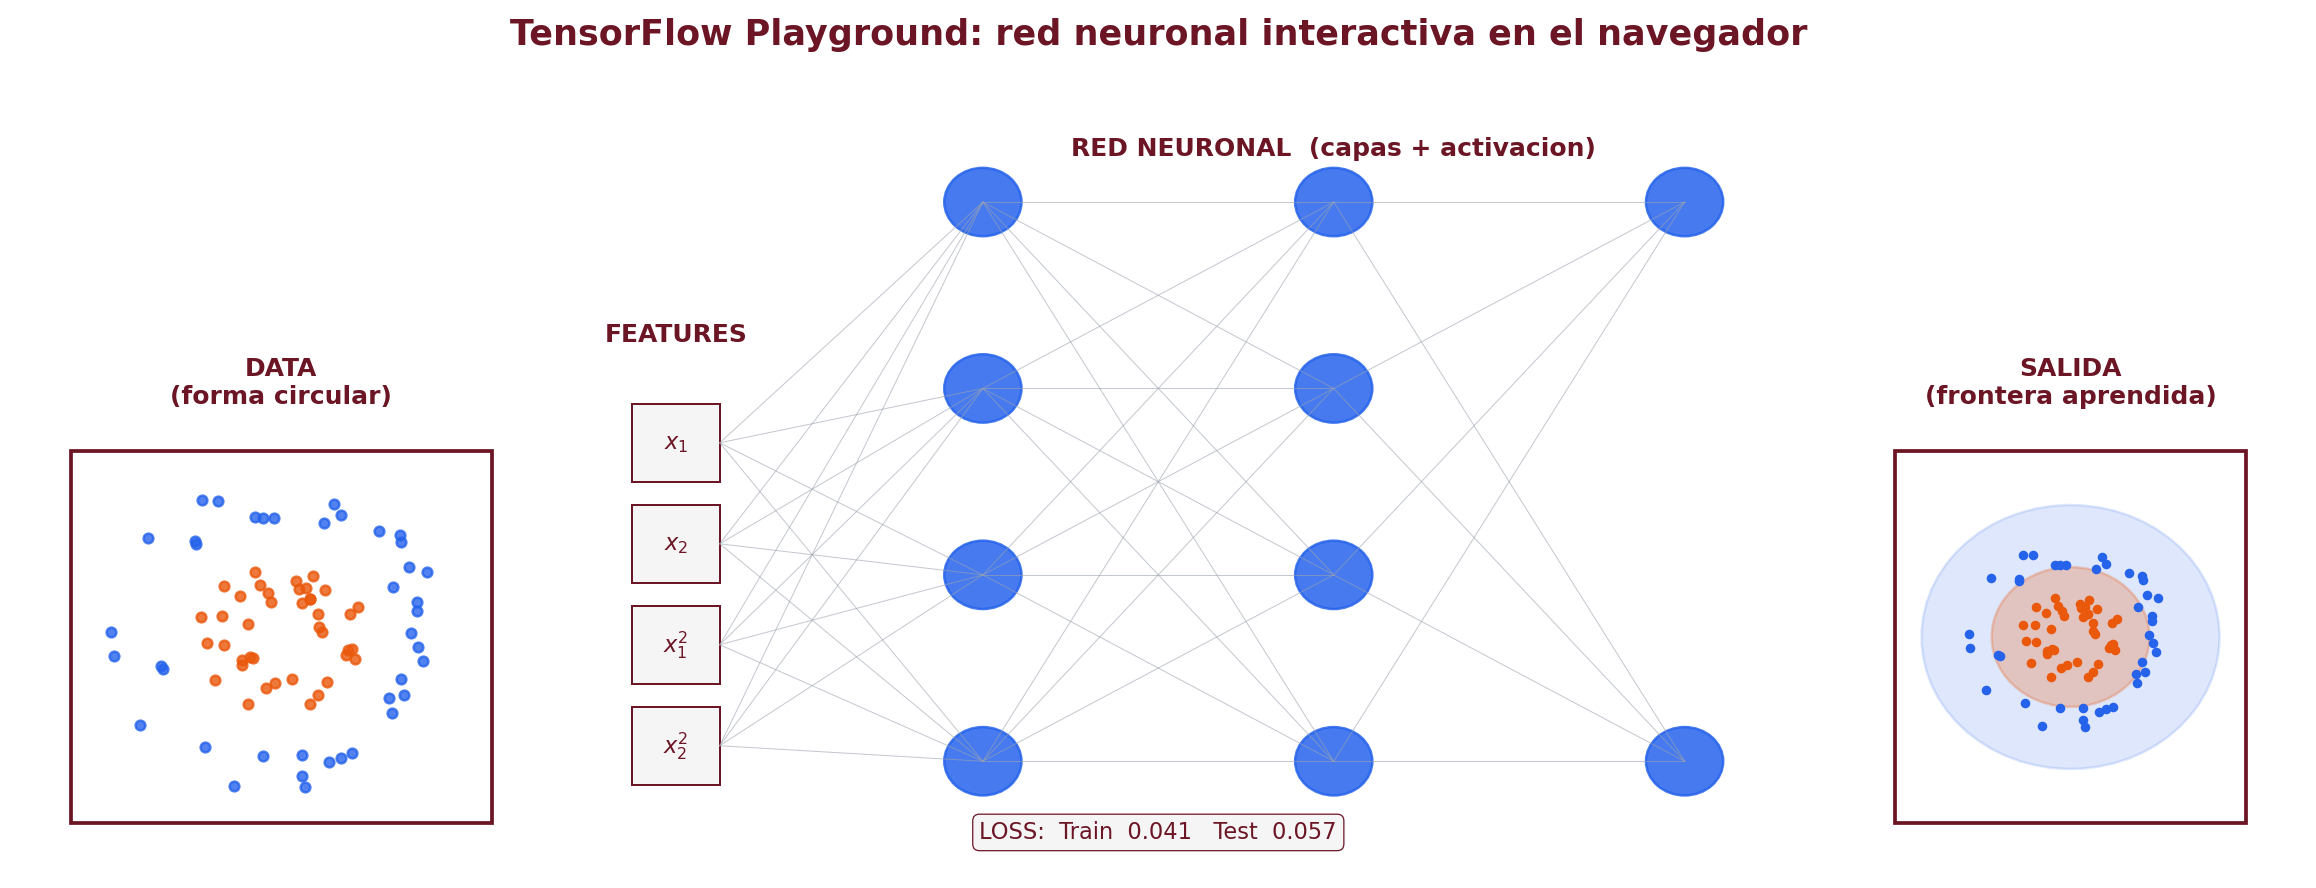
\includegraphics[width=0.92\textwidth]{fig_playground.png}
  \end{center}

  \vspace{4pt}
  {\footnotesize
  \textbf{URL:} \texttt{playground.tensorflow.org} --- gratis, sin instalar nada.}
\end{frame}

\begin{frame}[shrink]{Cuatro Experimentos en Vivo}
  \vspace{4pt}
  {\footnotesize\color{arcaDark}\bfseries
    Vamos al navegador. Cada experimento $\approx$ 3 minutos.}

  \vspace{8pt}
  {\footnotesize
  \begin{enumerate}\setlength{\itemsep}{8pt}
    \item[{\color{arcaRed}\bfseries 1.}]
      \textbf{C\'irculos} con $x_1, x_2$, 1 capa de 4, Tanh.
      \emph{Una capa con activaci\'on no lineal ya curva la frontera.}
    \item[{\color{arcaRed}\bfseries 2.}]
      \textbf{Espiral.} 1 capa de 8 (falla) $\to$ 3 capas de 8 (funciona).
      \emph{La profundidad importa cuando la frontera es compleja.}
    \item[{\color{arcaRed}\bfseries 3.}]
      Cambiar activaci\'on entre Sigmoid, Tanh, ReLU en la espiral.
      \emph{ReLU es la m\'as r\'apida y limpia.}
    \item[{\color{codeGreen}\bfseries 4.}]
      C\'irculos con \textbf{solo} $x_1^2$ y $x_2^2$ activados.
      \emph{Si las features son las correctas, una neurona basta.}
  \end{enumerate}
  }
\end{frame}

% =============================================================================
%  BLOQUE 2: LIMITACIONES DEL MLP
% =============================================================================
\sectionframe{?`Por Qu\'e el MLP No Puede con Im\'agenes?}{Tres problemas estructurales}

\begin{frame}[shrink]{Recordemos: Cats vs Dogs (Clase 22)}
  \vspace{4pt}
  {\footnotesize\color{arcaDark}\bfseries
    Aplicamos los mismos modelos a CIFAR-10 (32$\times$32 RGB).
    El resultado fue \textbf{una pared}, no un techo:}

  \vspace{16pt}
  \begin{center}
  {\footnotesize
  \begin{tabular}{@{}l c c c@{}}
    \toprule
    & \textbf{MNIST} & \textbf{Fashion MNIST} & \textbf{Cats vs Dogs (RGB)} \\
    \midrule
    Logistic       & 92\% & 84\% & \textbf{\color{arcaRed}55\%} \\
    Random Forest  & 95\% & 87\% & \textbf{\color{arcaRed}62\%} \\
    MLP (128, 64)  & 97\% & 88\% & \textbf{\color{arcaRed}60\%} \\
    \bottomrule
  \end{tabular}
  }
  \end{center}

  \vspace{16pt}
  {\footnotesize\color{arcaDark}
    Aumentar capacidad (m\'as capas, m\'as neuronas) \textbf{no rompe la pared}.
    No es un bug. Es un l\'imite \emph{estructural} del MLP. Vamos a ver
    exactamente cu\'al.}
\end{frame}

\begin{frame}[shrink]{Problema 1: No Es Invariante a Traslaci\'on}
  \vspace{4pt}
  {\footnotesize\color{arcaDark}\bfseries
    Mover un d\'igito \textbf{1 pixel} cambia el vector aplanado por completo.
    Para el MLP es \emph{otra} entrada.}

  \vspace{8pt}
  \begin{center}
    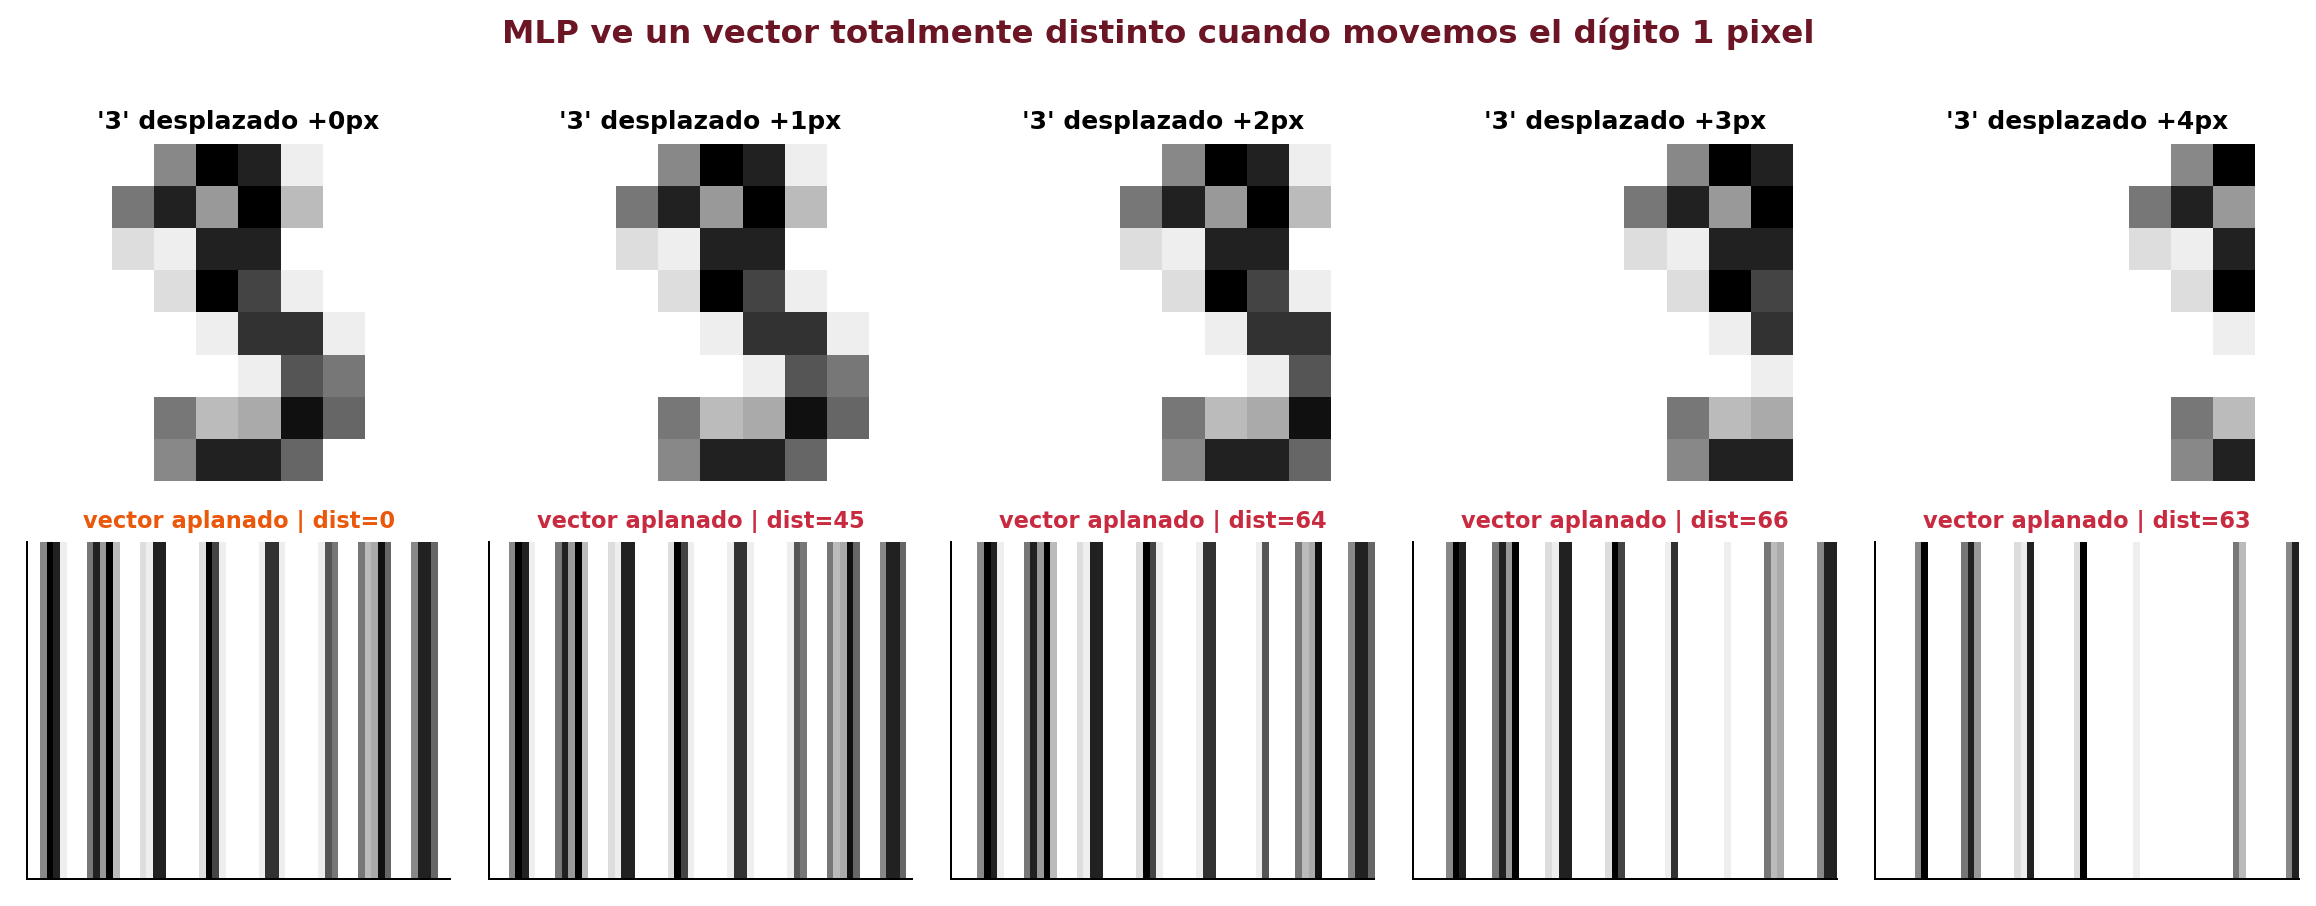
\includegraphics[width=0.92\textwidth]{fig_mlp_traslacion.png}
  \end{center}

  \vspace{4pt}
  {\scriptsize\color{textMuted}
    \faLightbulb\hspace{4pt} El MLP tendr\'ia que aprender ``ese 3''
    para cada posici\'on posible.}
\end{frame}

\begin{frame}[shrink]{Problema 2: Explosi\'on de Par\'ametros}
  \vspace{4pt}
  {\footnotesize\color{arcaDark}\bfseries
    Cada pixel se conecta con cada neurona. Con im\'agenes reales,
    el conteo se vuelve absurdo:}

  \vspace{8pt}
  \begin{center}
    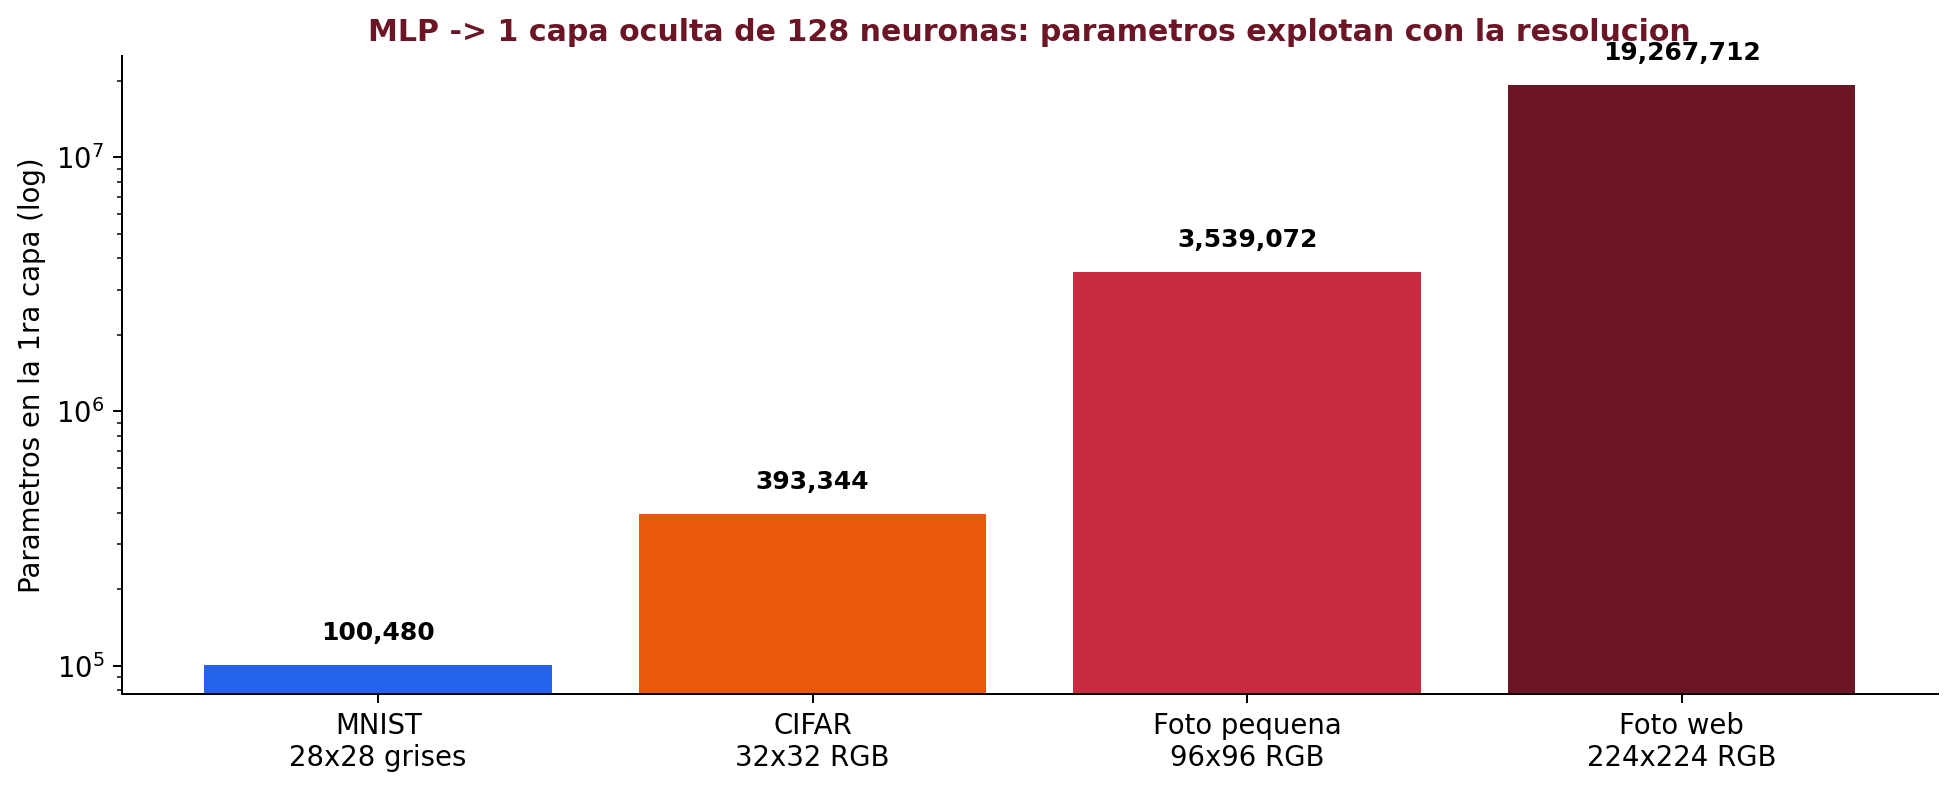
\includegraphics[width=0.85\textwidth]{fig_mlp_parametros.png}
  \end{center}

  \vspace{4pt}
  {\scriptsize\color{textMuted}
    \faLightbulb\hspace{4pt} Una sola capa de 128 neuronas para una foto
    $224\times224\times3$ requiere \textbf{19 millones} de pesos.}
\end{frame}

\begin{frame}[shrink]{Problema 3: Ignora la Estructura Espacial}
  \vspace{6pt}
  {\footnotesize\color{arcaDark}\bfseries
    El \texttt{.flatten()} convierte la imagen en un vector. Se pierde
    algo cr\'itico: \textbf{los pixeles vecinos est\'an relacionados}.}

  \vspace{14pt}
  {\footnotesize
  \begin{itemize}\setlength{\itemsep}{8pt}
    \item[{\color{arcaRed}\scriptsize\faArrowRight}]
      Pixel 100 y 101 est\'an \emph{lado a lado} en la imagen,
      pero para el MLP son ``columna 100'' y ``columna 101'' ---
      sin relaci\'on especial.
    \item[{\color{arcaRed}\scriptsize\faArrowRight}]
      Lo que define un \textbf{borde} o una \textbf{textura} es una
      relaci\'on \emph{local} entre pocos pixeles vecinos.
    \item[{\color{arcaRed}\scriptsize\faArrowRight}]
      Para el MLP, una imagen rotada 90$^\circ$ es \emph{otra} imagen.
  \end{itemize}
  }
\end{frame}

\begin{frame}[shrink]{?`Para Qu\'e Sirve el MLP Hoy en D\'ia?}
  \vspace{4pt}
  {\footnotesize\color{arcaDark}\bfseries
    Sigue siendo \'util, pero su nicho se hizo angosto:}

  \vspace{14pt}
  {\footnotesize
  \begin{tabular}{@{}p{6.4cm} p{6.4cm}@{}}
    \toprule
    \textbf{\color{codeGreen}MLP est\'a OK cuando\ldots} & \textbf{\color{arcaRed}NO usar MLP cuando\ldots} \\
    \midrule
    Datos tabulares peque\~nos ($<$ 100 features). & Im\'agenes (CNN o ViT). \\
    Cabezal final de una CNN o Transformer. & Audio / espectrogramas. \\
    Prototipado r\'apido para validar ML. & Texto (Transformers / LLMs). \\
    \bottomrule
  \end{tabular}
  }

  \vspace{14pt}
  \begin{tcolorbox}[colback=arcaGray, colframe=arcaRed, boxrule=0.5pt,
    arc=2pt, left=6pt, right=6pt, top=4pt, bottom=4pt]
    {\scriptsize\color{arcaDark}
    \faKey\hspace{4pt}\textbf{Realidad de 2026:} casi nadie entrena un MLP
    \emph{puro} a gran escala. Sigue vivo como \textbf{cabezal} de modelos
    m\'as grandes (CNN, Transformer). La pieza importante son las
    arquitecturas que vienen \emph{antes}.}
  \end{tcolorbox}
\end{frame}

% =============================================================================
%  BLOQUE 3: CONVOLUCION
% =============================================================================
\sectionframe{Convoluci\'on}{Construyamos el concepto paso a paso}

\begin{frame}[shrink]{Pausa: ?`Qu\'e Es Un ``Par\'ametro''?}
  \vspace{4pt}
  {\footnotesize\color{arcaDark}\bfseries
    Antes de seguir, fijemos un t\'ermino que usaremos mucho.}

  \vspace{8pt}
  \begin{center}
    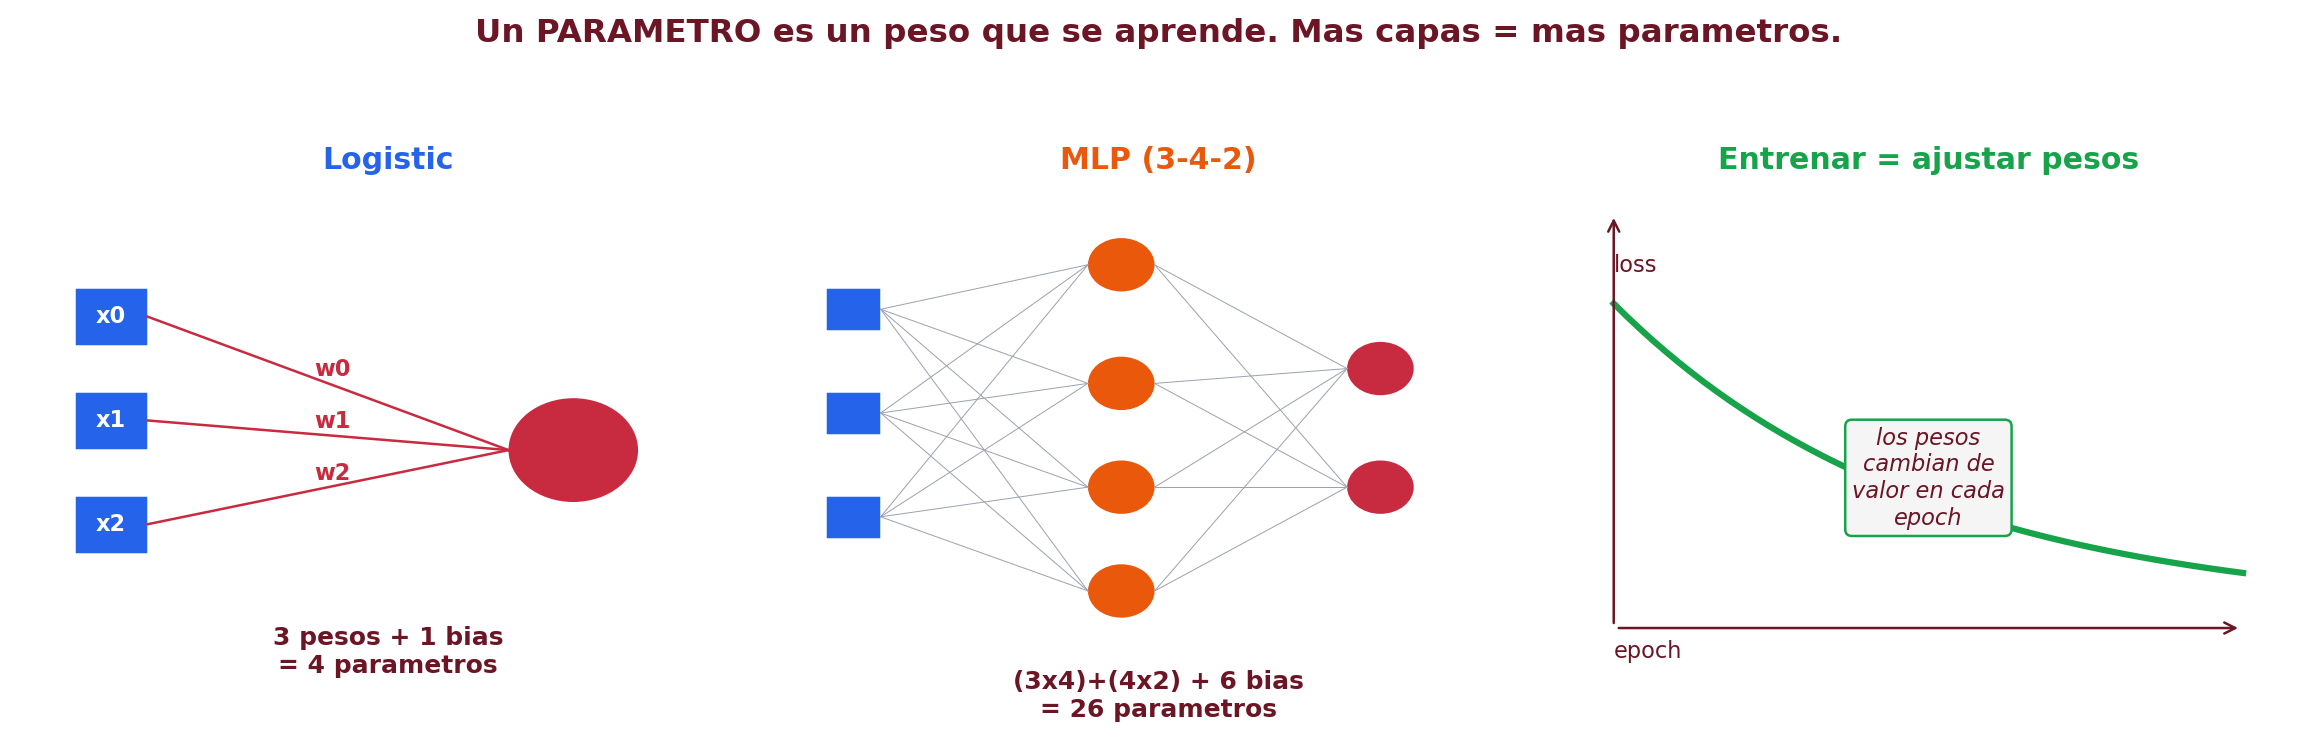
\includegraphics[width=0.92\textwidth]{fig_parametros.png}
  \end{center}

  \vspace{4pt}
  {\footnotesize
  \begin{itemize}\setlength{\itemsep}{2pt}
    \item[{\color{arcaRed}\scriptsize\faArrowRight}]
      \textbf{Un par\'ametro = un n\'umero (peso o bias) que se aprende
      durante el entrenamiento.}
    \item[{\color{arcaRed}\scriptsize\faArrowRight}]
      Cada \texttt{epoch}, el optimizador ajusta los par\'ametros para
      bajar el loss. \textbf{No los configuramos a mano.}
    \item[{\color{codeGreen}\scriptsize\faArrowRight}]
      M\'as par\'ametros = m\'as capacidad, pero \emph{tambi\'en} m\'as
      datos necesarios para que aprendan bien.
  \end{itemize}
  }
\end{frame}

\begin{frame}[shrink]{Empecemos por la Pieza B\'asica: Un Filtro}
  \vspace{6pt}
  {\footnotesize\color{arcaDark}\bfseries
    Un \textbf{filtro} (o \textbf{kernel}) es una matriz peque\~na de
    par\'ametros. Lo m\'as com\'un: una matriz \textbf{3$\times$3}.}

  \vspace{14pt}
  {\footnotesize
  \begin{itemize}\setlength{\itemsep}{6pt}
    \item[{\color{arcaRed}\scriptsize\faArrowRight}]
      Una matriz 3$\times$3 tiene \textbf{9 n\'umeros}: estos son los
      9 par\'ametros que la red va a aprender.
    \item[{\color{arcaRed}\scriptsize\faArrowRight}]
      Antes de las CNN, los ingenieros \emph{escrib\'ian a mano} los
      9 valores (filtros como Sobel para detectar bordes).
    \item[{\color{codeGreen}\scriptsize\faArrowRight}]
      En una CNN, esos 9 valores los \textbf{aprende el optimizador}
      a partir de los datos. Mismo c\'odigo, mucho mejor resultado.
  \end{itemize}
  }
\end{frame}

\begin{frame}[shrink]{La Operaci\'on, Paso a Paso (1/3): UNA Posici\'on}
  \vspace{4pt}
  {\footnotesize\color{arcaDark}\bfseries
    Veamos exactamente qu\'e pasa en \textbf{una sola posici\'on} de la
    ventana.}

  \vspace{14pt}
  \begin{center}
  \begin{tikzpicture}[
    cell/.style={rectangle, draw=arcaDark, line width=0.4pt, minimum size=0.7cm,
                 inner sep=0pt, font=\small\bfseries},
    inputc/.style={cell, fill=codeBlue!20, text=arcaDark},
    inputh/.style={cell, fill=codeBlue!50, text=white},
    kernelc/.style={cell, fill=codeOrange!30, text=arcaDark},
    outputc/.style={cell, fill=arcaRed!85, text=white, minimum size=1.2cm,
                    font=\Large\bfseries},
  ]
    % ─── INPUT 5x5 with first 3x3 window highlighted ───
    \node[font=\bfseries\color{codeBlue}, anchor=south] at (1.4, 3.7) {INPUT 5$\times$5};
    \def\inp{{{3,1,2,7,5},{0,1,1,4,8},{1,2,2,0,1},{3,9,8,0,0},{4,8,1,5,4}}}
    \foreach \i in {0,...,4}{
      \foreach \j in {0,...,4}{
        \pgfmathtruncatemacro{\v}{\inp[\i][\j]}
        \ifnum\i<3 \ifnum\j<3
          \node[inputh] at (\j*0.7, 3.0 - \i*0.7) {\v};
        \else \node[inputc] at (\j*0.7, 3.0 - \i*0.7) {\v}; \fi
        \else \node[inputc] at (\j*0.7, 3.0 - \i*0.7) {\v}; \fi
      }
    }
    \draw[arcaRed, line width=2pt]
      (-0.35, 3.35) rectangle (1.75, 1.25);
    \node[font=\scriptsize\color{arcaRed}\bfseries, anchor=north]
      at (0.7, 0.85) {ventana 3$\times$3};

    % ─── KERNEL 3x3 ───
    \node[font=\bfseries\color{codeOrange}, anchor=south] at (5.6, 3.7) {FILTRO};
    \def\ker{{{1,0,-1},{1,0,-1},{1,0,-1}}}
    \foreach \i in {0,...,2}{
      \foreach \j in {0,...,2}{
        \pgfmathtruncatemacro{\v}{\ker[\i][\j]}
        \node[kernelc] at (4.9 + \j*0.7, 3.0 - \i*0.7) {\v};
      }
    }

    % ─── Operation in middle ───
    \node[font=\Large\bfseries\color{arcaDark}] at (3.4, 2.3) {$\bigodot$};
    \node[font=\scriptsize\color{textMuted}] at (3.4, 1.6) {multiplicar};
    \node[font=\scriptsize\color{textMuted}] at (3.4, 1.3) {elemento a};
    \node[font=\scriptsize\color{textMuted}] at (3.4, 1.0) {elemento};

    % ─── Sum + arrow to output ───
    \node[font=\Large\bfseries\color{arcaDark}] at (7.6, 2.3) {$\sum$};
    \node[font=\scriptsize\color{textMuted}] at (7.6, 1.6) {sumar};
    \node[font=\scriptsize\color{textMuted}] at (7.6, 1.3) {los 9};

    % ─── Detail of products ───
    \node[font=\tiny\color{arcaDark}, anchor=west, text width=4cm] at (8.4, 3.3)
      {$3{\cdot}1 + 1{\cdot}0 + 2{\cdot}({-}1)$\\
       $+\; 0{\cdot}1 + 1{\cdot}0 + 1{\cdot}({-}1)$\\
       $+\; 1{\cdot}1 + 2{\cdot}0 + 2{\cdot}({-}1)$};
    \draw[->, line width=1pt, arcaDark] (10.5, 2.7) -- (11.6, 2.5);

    % ─── Output value ───
    \node[outputc] at (12.2, 2.5) {-1};
    \node[font=\bfseries\color{white}, anchor=south, font=\scriptsize] at (12.2, 3.3) {1 numero};
  \end{tikzpicture}
  \end{center}

  \vspace{8pt}
  {\scriptsize\color{textMuted}
    \faLightbulb\hspace{4pt} \textbf{En una posici\'on:} 9
    multiplicaciones, sumar los 9 productos $\Rightarrow$ \textbf{1 solo
    n\'umero} de salida. Aqu\'i: $3{\cdot}1 + 1{\cdot}0 + 2{\cdot}({-}1) +
    \ldots = -1$.}
\end{frame}

\begin{frame}[shrink]{La Operaci\'on, Paso a Paso (2/3): Deslizar}
  \vspace{4pt}
  {\footnotesize\color{arcaDark}\bfseries
    Para llenar el resto de la salida, \textbf{deslizamos} la ventana
    de a 1 pixel y repetimos. La salida completa = \textbf{mapa de
    caracter\'isticas} (\emph{feature map}).}

  \vspace{14pt}
  \begin{center}
  \begin{tikzpicture}[
    cell/.style={rectangle, draw=arcaDark!50, line width=0.3pt,
                 minimum size=0.55cm, inner sep=0pt, font=\scriptsize\bfseries},
    inputc/.style={cell, fill=codeBlue!15, text=arcaDark},
    inputh/.style={cell, fill=codeBlue!55, text=white},
    outc/.style={cell, fill=arcaRed!85, text=white},
    outempty/.style={cell, fill=arcaRed!10, text=arcaRed!50},
  ]
    % Input 5x5 with window at 3 different positions, shown 3 times
    \def\inp{{{3,1,2,7,5},{0,1,1,4,8},{1,2,2,0,1},{3,9,8,0,0},{4,8,1,5,4}}}

    % Helper to draw input
    \foreach \frame/\posi/\posj/\xoff/\out/\filled in {%
      1/0/0/0/-1/0,
      2/0/1/4.7/-7/1,
      3/1/0/9.4/-7/2}{
      % Title
      \node[font=\bfseries\color{arcaDark}, anchor=south]
        at (\xoff + 1.4, 3.6) {Paso \frame};
      % Input grid
      \foreach \i in {0,...,4}{
        \foreach \j in {0,...,4}{
          \pgfmathtruncatemacro{\v}{\inp[\i][\j]}
          \pgfmathtruncatemacro{\inwin}{(\i>=\posi && \i<\posi+3 && \j>=\posj && \j<\posj+3)?1:0}
          \ifnum\inwin=1
            \node[inputh] at (\xoff + \j*0.55, 3.0 - \i*0.55) {\v};
          \else
            \node[inputc] at (\xoff + \j*0.55, 3.0 - \i*0.55) {\v};
          \fi
        }
      }
      % Window highlight
      \draw[arcaRed, line width=1.2pt]
        (\xoff + \posj*0.55 - 0.275, 3.275 - \posi*0.55) rectangle
        (\xoff + \posj*0.55 + 1.375, 3.275 - \posi*0.55 - 1.65);

      % Mini output 3x3 next to it
      \foreach \oi in {0,...,2}{
        \foreach \oj in {0,...,2}{
          \pgfmathtruncatemacro{\f}{\filled}
          \pgfmathtruncatemacro{\here}{(\oi==\posi && \oj==\posj)?1:0}
          \pgfmathtruncatemacro{\done}{(\oi*3+\oj < \f)?1:0}
          \ifnum\here=1
            \node[outc] at (\xoff + 3.4 + \oj*0.4, 2.5 - \oi*0.4) {\out};
          \else
            \ifnum\done=1
              \node[outc, fill=arcaRed!50] at (\xoff + 3.4 + \oj*0.4, 2.5 - \oi*0.4) {};
            \else
              \node[outempty] at (\xoff + 3.4 + \oj*0.4, 2.5 - \oi*0.4) {?};
            \fi
          \fi
        }
      }
    }

    \node[font=\scriptsize\color{textMuted}, anchor=north]
      at (6.0, 0.5) {ventana 3$\times$3 \emph{recorre} todas las posiciones del input $\to$ output 3$\times$3};
  \end{tikzpicture}
  \end{center}

  \vspace{6pt}
  {\scriptsize\color{textMuted}
    \faLightbulb\hspace{4pt} 9 posiciones distintas de la ventana
    $\Rightarrow$ 9 n\'umeros en el output. La salida completa es la
    \textbf{respuesta del filtro} en toda la imagen.}
\end{frame}

\begin{frame}[shrink]{La Operaci\'on, Paso a Paso (3/3)}
  \vspace{4pt}
  {\footnotesize\color{arcaDark}\bfseries
    Una imagen de \textbf{5$\times$5} con un filtro \textbf{3$\times$3}
    produce una salida de \textbf{3$\times$3}. (Veremos despu\'es c\'omo
    conservar el tama\~no con \emph{padding}.)}

  \vspace{14pt}
  {\footnotesize
  \begin{itemize}\setlength{\itemsep}{6pt}
    \item[{\color{arcaRed}\scriptsize\faArrowRight}]
      \textbf{En cada posici\'on:} 9 multiplicaciones + 1 suma.
    \item[{\color{arcaRed}\scriptsize\faArrowRight}]
      \textbf{En total} (5$\times$5 con filtro 3$\times$3): 9 posiciones
      del output, $\sim$80 operaciones.
    \item[{\color{arcaRed}\scriptsize\faArrowRight}]
      \textbf{En una imagen real} (32$\times$32 con 32 filtros):
      $\sim$280\,000 operaciones para una sola capa Conv2D.
    \item[{\color{codeGreen}\scriptsize\faArrowRight}]
      Por eso necesitamos GPU. Lo veremos en el bloque 4.
  \end{itemize}
  }
\end{frame}

\begin{frame}[shrink]{?`Por Qu\'e Se Llama ``Convoluci\'on''?}
  \vspace{4pt}
  {\footnotesize\color{arcaDark}\bfseries
    El nombre viene de matem\'aticas, no de visi\'on por computadora.
    Es una operaci\'on cl\'asica de \textbf{procesamiento de se\~nales}
    que existe desde el siglo XVIII.}

  \vspace{6pt}
  \begin{center}
    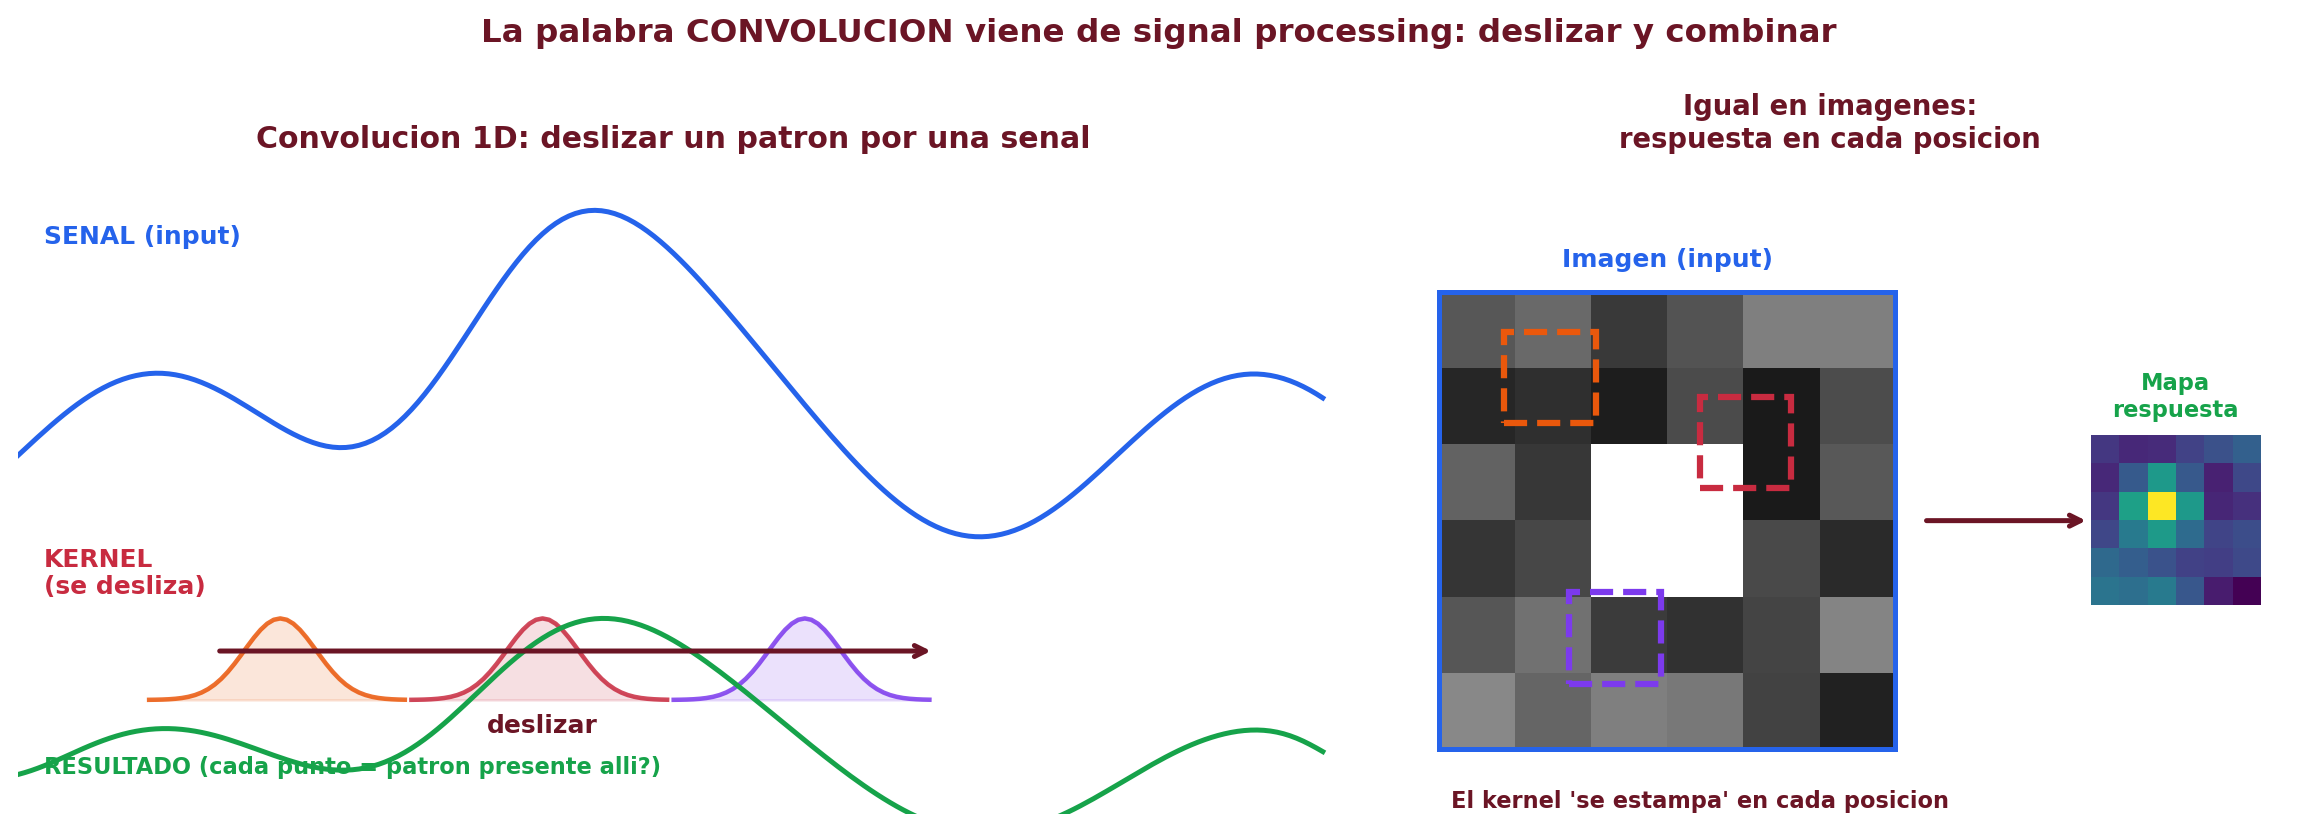
\includegraphics[width=0.95\textwidth]{fig_conv_origen.png}
  \end{center}

  \vspace{4pt}
  {\scriptsize\color{textMuted}
    \faLightbulb\hspace{4pt} En \textbf{audio}: el eco de una sala se
    modela con convoluci\'on (filtro = patr\'on de eco).
    En \textbf{sensores}: suavizar una se\~nal ruidosa
    (filtro = promedio m\'ovil). La idea de \emph{deslizar y combinar}
    es la misma --- en 1D para se\~nales, en 2D para im\'agenes.}
\end{frame}

\begin{frame}[shrink]{?`Qu\'e ``Buscan'' los Filtros? --- Filtros a Mano}
  \vspace{4pt}
  {\footnotesize\color{arcaDark}\bfseries
    Antes de las CNN ya se sab\'ia que un filtro es un \textbf{detector
    de patrones}. El cl\'asico ejemplo: el filtro \textbf{Sobel}
    detecta bordes con apenas 9 n\'umeros escritos a mano.}

  \vspace{6pt}
  \begin{center}
    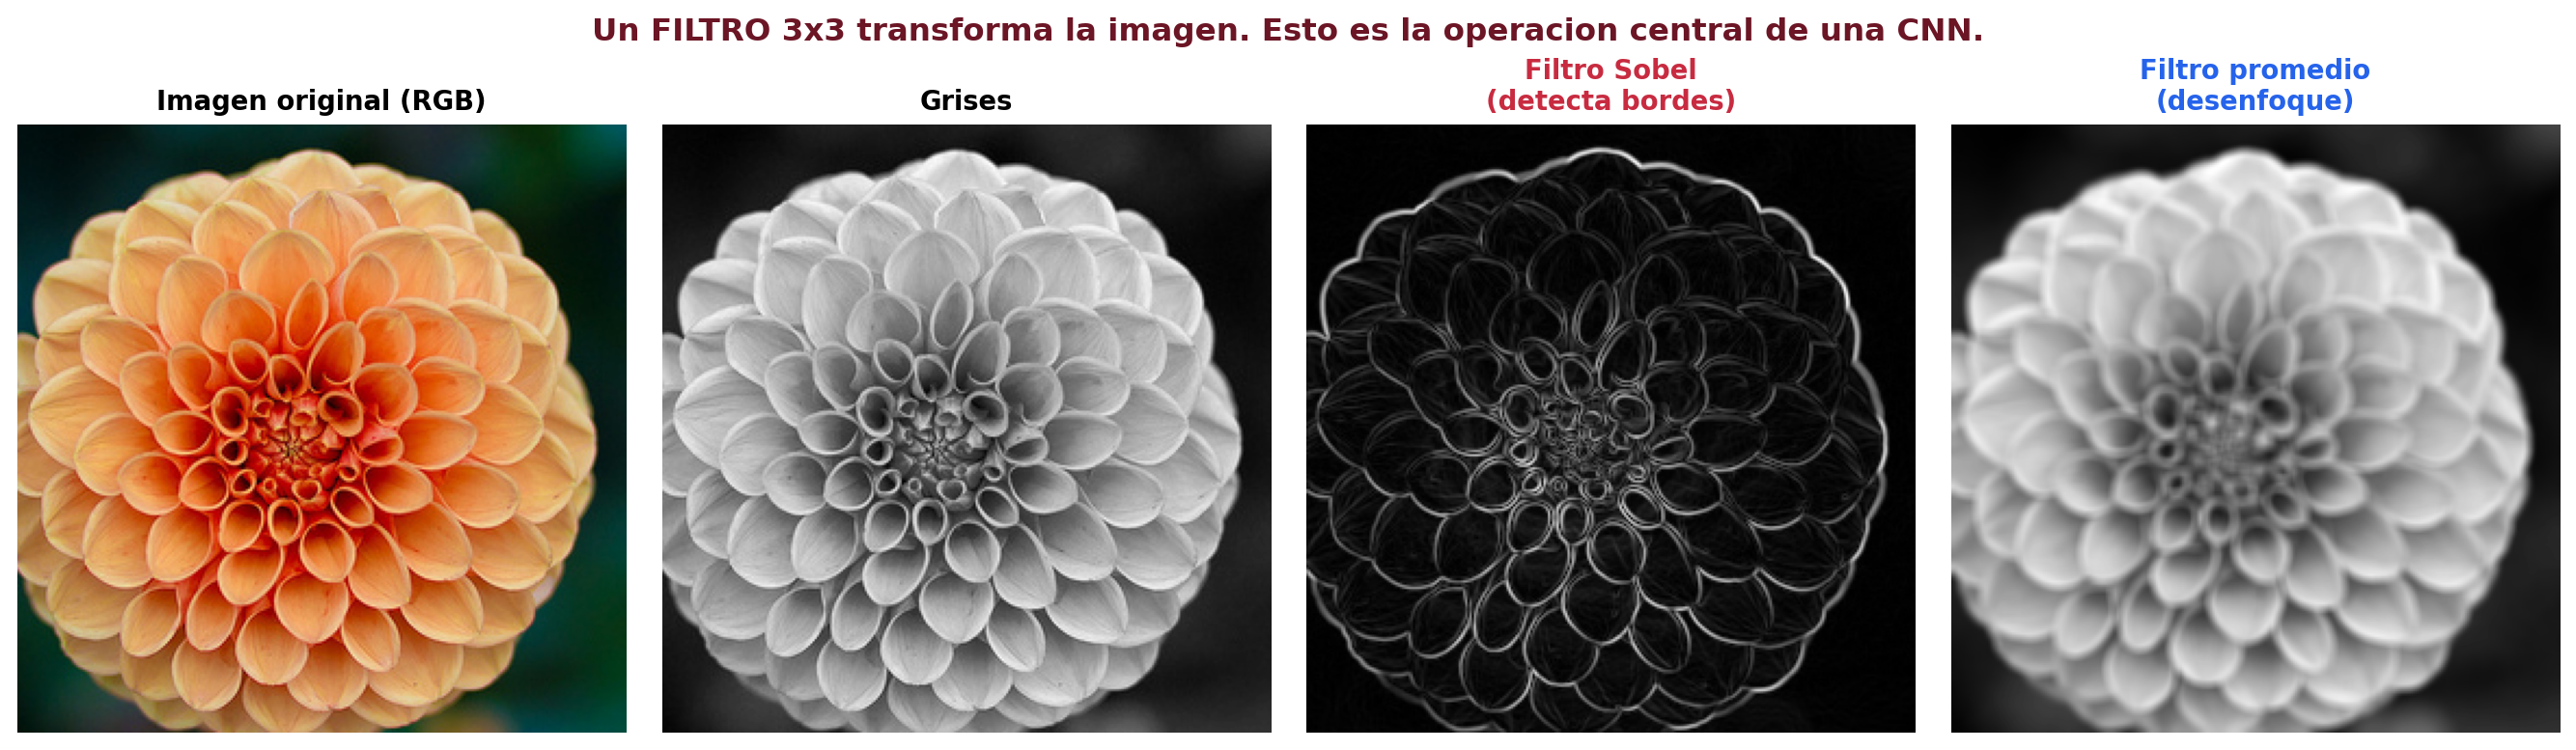
\includegraphics[width=0.95\textwidth]{fig_filtro_edge.png}
  \end{center}

  \vspace{2pt}
  {\scriptsize\color{textMuted}
    \faLightbulb\hspace{4pt} \textbf{Sobel} (Stanford, 1968): patr\'on
    \texttt{[[-1,0,1],[-2,0,2],[-1,0,1]]}. La salida brilla donde
    hay un cambio brusco de izquierda a derecha (un borde vertical).}
\end{frame}

\begin{frame}[shrink]{?`Qu\'e Hace una CNN Distinto? --- Filtros Aprendidos}
  \vspace{8pt}
  {\footnotesize\color{arcaDark}\bfseries
    Una CNN \textbf{no} usa filtros a mano. Empieza con valores
    aleatorios y los \textbf{aprende} por descenso de gradiente,
    igual que cualquier otra red.}

  \vspace{14pt}
  {\footnotesize
  \begin{itemize}\setlength{\itemsep}{6pt}
    \item[{\color{arcaRed}\scriptsize\faArrowRight}]
      Una capa Conv2D no usa \emph{un} filtro: usa \textbf{decenas}
      (32, 64, 128\ldots) en paralelo.
    \item[{\color{arcaRed}\scriptsize\faArrowRight}]
      Cada filtro se especializa en un patr\'on distinto: bordes en
      \'angulos, manchas, esquinas, texturas\ldots
    \item[{\color{codeGreen}\scriptsize\faArrowRight}]
      \textbf{Cu\'al patr\'on aprende cada filtro lo decide el optimizador}
      buscando minimizar el loss. Para nuestro problema concreto.
  \end{itemize}
  }
\end{frame}

\begin{frame}[shrink]{Muchos Filtros = Muchos Mapas de Caracter\'isticas}
  \vspace{4pt}
  \begin{center}
    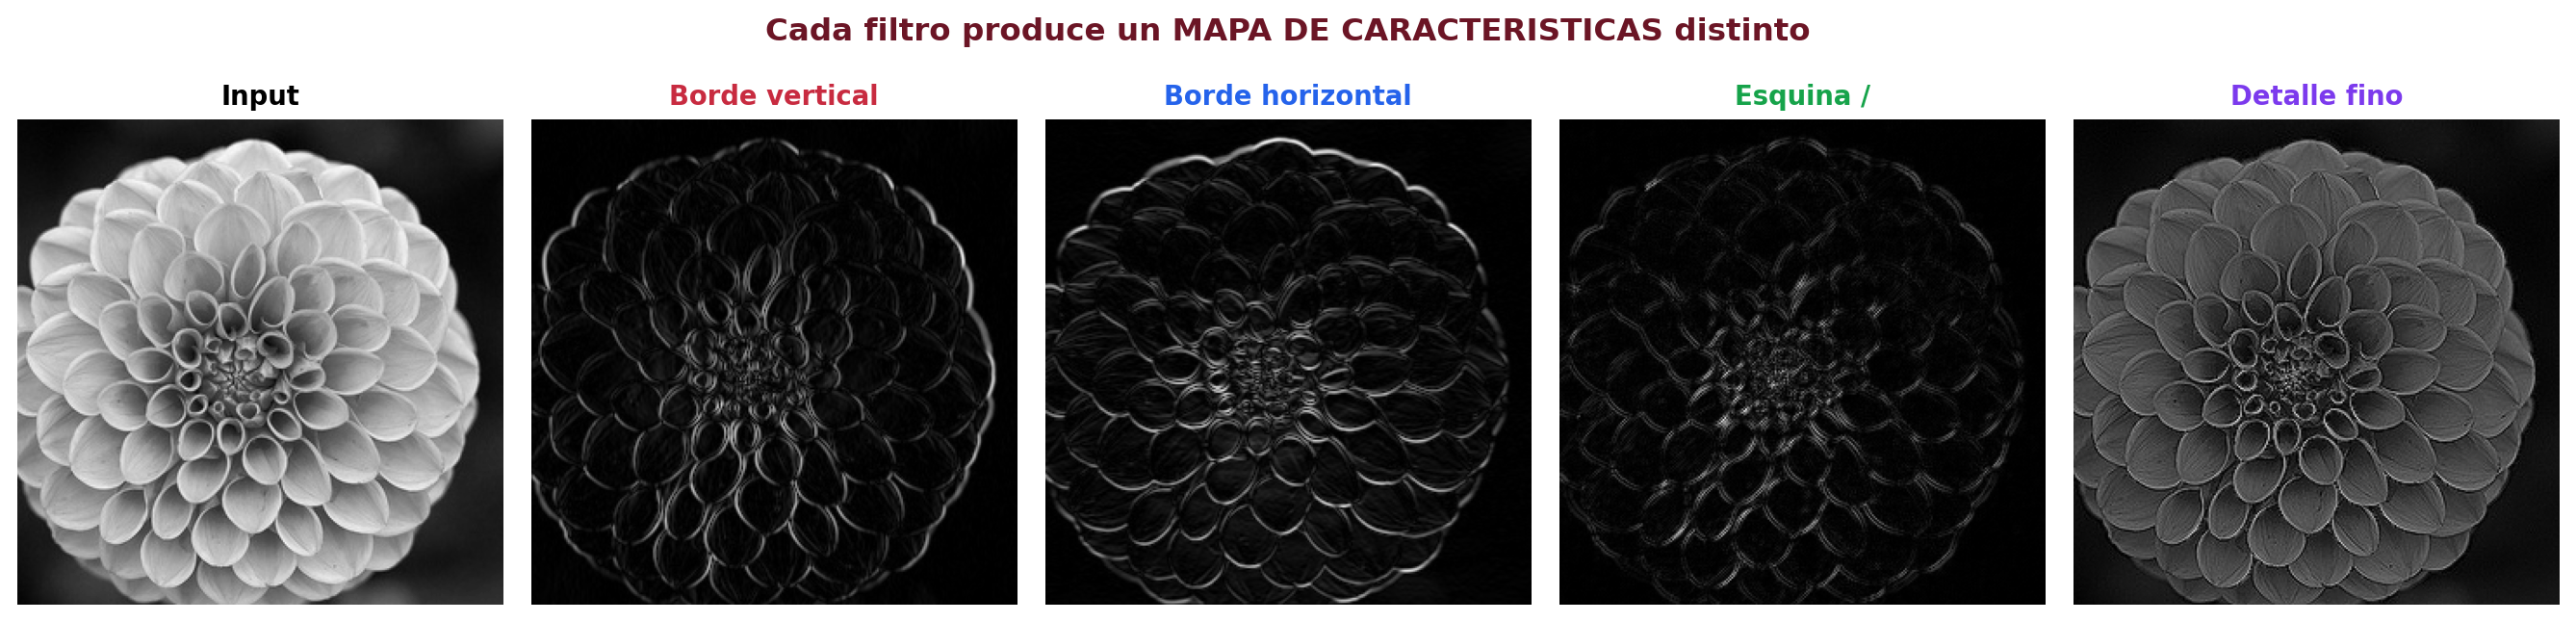
\includegraphics[width=0.95\textwidth]{fig_feature_maps.png}
  \end{center}

  \vspace{4pt}
  {\scriptsize\color{textMuted}
    \faLightbulb\hspace{4pt} Si la capa tiene \textbf{32 filtros},
    la salida tiene \textbf{32 canales} (32 ``versiones'' de la
    imagen, cada una resaltando un patr\'on distinto). La siguiente
    capa Conv2D recibe esos 32 canales como entrada.}
\end{frame}

\begin{frame}[shrink]{Por Qu\'e Esto Resuelve los 3 Problemas del MLP}
  \vspace{8pt}
  {\footnotesize
  \begin{tabular}{@{}p{3.8cm} p{8.5cm}@{}}
    \toprule
    \textbf{Problema MLP} & \textbf{C\'omo lo resuelve la convoluci\'on} \\
    \midrule
    \rowcolor{arcaGray}
    Traslaci\'on cambia todo
    & El \emph{mismo} filtro se aplica en \emph{cada} posici\'on. Si
      detecta un borde aqu\'i, lo detecta all\'a. \\
    Explosi\'on de par\'ametros
    & Solo 9 par\'ametros por filtro, sin importar el tama\~no de la
      imagen (\textbf{parameter sharing}). \\
    \rowcolor{arcaGray}
    Ignora estructura espacial
    & La ventana 3$\times$3 mira pixeles \emph{vecinos} ---
      la geometr\'ia local est\'a integrada. \\
    \bottomrule
  \end{tabular}
  }

  \vspace{14pt}
  \begin{tcolorbox}[colback=codeGreen!8, colframe=codeGreen, boxrule=0.5pt,
    arc=2pt, left=6pt, right=6pt, top=4pt, bottom=4pt]
    {\scriptsize\color{arcaDark}
    \faKey\hspace{4pt}\textbf{La convoluci\'on no es magia:} es una
    operaci\'on b\'asica (multiplicar y sumar) aplicada con el truco de
    \emph{compartir los par\'ametros}. Esa simplicidad es lo que la
    hace funcionar.}
  \end{tcolorbox}
\end{frame}

% =============================================================================
%  BLOQUE 4: ANATOMIA DE UNA CNN
% =============================================================================
\sectionframe{Anatom\'ia de una CNN}{Las 3 etapas y por qu\'e cada una}

\begin{frame}[shrink]{Toda CNN Tiene 3 Etapas}
  \vspace{4pt}
  {\footnotesize\color{arcaDark}\bfseries
    Antes de mirar capa por capa, veamos la estructura general.
    \textbf{Toda CNN, sin excepci\'on, tiene estas 3 etapas en este orden}:}

  \vspace{12pt}
  \begin{center}
  \begin{tikzpicture}[
    stage/.style={rectangle, rounded corners=4pt, minimum width=4cm,
                  minimum height=4cm, align=center, text width=3.7cm,
                  font=\footnotesize, inner sep=8pt},
    title/.style={rectangle, rounded corners=4pt, minimum width=4cm,
                  minimum height=0.7cm, align=center, font=\small\bfseries\color{white}},
  ]
    % ETAPA 1
    \node[title, fill=codeBlue] (t1) {ETAPA 1: extraer features};
    \node[stage, fill=arcaGray, draw=codeBlue, line width=1.2pt,
          below=2pt of t1] (b1)
      {{\bfseries\color{arcaDark}Conv2D + ReLU + MaxPool}\\[2pt]
       {\scriptsize(repetir 2--4 veces)}\\[6pt]
       {\bfseries\color{arcaDark}p\'ixeles $\to$ bordes}\\
       {\bfseries\color{arcaDark}$\to$ texturas $\to$ partes}\\[6pt]
       {\scriptsize\itshape\color{textMuted}Filtros 3$\times$3 detectan patrones.}\\
       {\scriptsize\itshape\color{textMuted}MaxPool reduce el tama\~no.}};

    % ETAPA 2
    \node[title, fill=codePurple, right=8pt of t1] (t2) {ETAPA 2: aplanar};
    \node[stage, fill=arcaGray, draw=codePurple, line width=1.2pt,
          below=2pt of t2] (b2)
      {{\bfseries\color{arcaDark}Flatten}\\[12pt]
       {\bfseries\color{arcaDark}Tensor 3D}\\
       {\bfseries\color{arcaDark}$\to$ vector 1D}\\[12pt]
       {\scriptsize\itshape\color{textMuted}Solo cambia la forma.}\\
       {\scriptsize\itshape\color{textMuted}Sin par\'ametros.}};

    % ETAPA 3
    \node[title, fill=arcaRed, right=8pt of t2] (t3) {ETAPA 3: clasificar};
    \node[stage, fill=arcaGray, draw=arcaRed, line width=1.2pt,
          below=2pt of t3] (b3)
      {{\bfseries\color{arcaDark}Dense + ReLU}\\
       {\bfseries\color{arcaDark}Dense + Softmax}\\[8pt]
       {\bfseries\color{arcaDark}El ``cerebro''}\\
       {\bfseries\color{arcaDark}que decide}\\[8pt]
       {\scriptsize\itshape\color{textMuted}MLP cl\'asico al final.}\\
       {\scriptsize\itshape\color{textMuted}Una decisi\'on por clase.}};

    % Arrows
    \draw[->, line width=1.2pt, arcaDark] (b1.east) -- (b2.west);
    \draw[->, line width=1.2pt, arcaDark] (b2.east) -- (b3.west);
  \end{tikzpicture}
  \end{center}

  \vspace{4pt}
  {\scriptsize\color{textMuted}
    \faLightbulb\hspace{4pt} Las 4 capas que vamos a estudiar se
    reparten en estas 3 etapas. Vamos a verlas en orden.}
\end{frame}

\begin{frame}{Etapa 1, Capa A: \texttt{Conv2D}}
  \vspace{4pt}
  {\footnotesize\color{arcaDark}\bfseries
    Aplica los filtros de los que hablamos. Tiene tres argumentos clave:}

  \vspace{14pt}
  {\footnotesize
  \begin{tabular}{@{}p{2.6cm} p{4.3cm} p{5.5cm}@{}}
    \toprule
    \textbf{Argumento} & \textbf{Qu\'e controla} & \textbf{Qu\'e elegir} \\
    \midrule
    \rowcolor{arcaGray}
    \texttt{filters}
    & Cu\'antos filtros aprende. Cada filtro produce 1 mapa de salida.
    & Empezar 32 o 64. \\
    \texttt{kernel\_size}
    & Tama\~no de cada filtro.
    & \textbf{3} casi siempre. \\
    \rowcolor{arcaGray}
    \texttt{padding}
    & Qu\'e pasa con los bordes.
    & \textbf{``same''} para conservar tama\~no. \\
    \bottomrule
  \end{tabular}
  }

  \vspace{14pt}
  {\footnotesize\color{arcaDark}
    \faLightbulb\hspace{4pt} \texttt{Conv2D(64, 3, padding="same",
    activation="relu")} se lee: ``64 filtros 3$\times$3 que conservan
    el tama\~no espacial, seguidos de ReLU''.}
\end{frame}

\begin{frame}{Detalle: ?`Qu\'e es el \emph{Padding}?}
  \vspace{4pt}
  {\footnotesize\color{arcaDark}\bfseries
    Cuando una ventana 3$\times$3 recorre la imagen, no puede llegar
    hasta los bordes (la ventana se sale). \textbf{Padding} es agregar
    una orilla de ceros para que la ventana s\'i pueda llegar.}

  \vspace{14pt}
  \begin{center}
  \begin{tikzpicture}[
    cell/.style={rectangle, draw=white, line width=0.4pt, minimum size=0.5cm,
                 inner sep=0pt, font=\tiny},
    inputc/.style={cell, fill=codeBlue!75, text=white},
    outputc/.style={cell, fill=arcaRed!75, text=white},
    padc/.style={cell, fill=textMuted!30},
  ]
    % ─── Left: padding=valid ───
    \node[font=\bfseries\color{arcaRed}] at (1.5, 4.0) {padding="valid" (sin padding)};
    % Input 5x5
    \foreach \i in {0,...,4}{
      \foreach \j in {0,...,4}{
        \node[inputc] at (\j*0.5, 3.0 - \i*0.5) {};
      }
    }
    \node[font=\bfseries\color{white}] at (1.0, 2.0) {INPUT 5$\times$5};
    % Arrow
    \draw[->, line width=1.5pt, arcaDark] (3.0, 1.5) -- (3.7, 1.5);
    % Output 3x3
    \foreach \i in {0,...,2}{
      \foreach \j in {0,...,2}{
        \node[outputc] at (4.0 + \j*0.5, 2.5 - \i*0.5) {};
      }
    }
    \node[font=\bfseries\color{white}] at (4.5, 2.0) {OUT 3$\times$3};
    \node[font=\scriptsize\color{textMuted}, text width=4cm, align=center] at (3.0, 0.0)
      {Output \textbf{m\'as chico}.\\Las esquinas se ``pierden''.};

    % ─── Right: padding=same ───
    \node[font=\bfseries\color{codeGreen}] at (10.0, 4.0) {padding="same" (rodear con ceros)};
    % Padding ring (7x7)
    \foreach \i in {0,...,6}{
      \foreach \j in {0,...,6}{
        \node[padc] at (8.0 + \j*0.5, 3.5 - \i*0.5) {};
      }
    }
    % Input 5x5 over padding
    \foreach \i in {0,...,4}{
      \foreach \j in {0,...,4}{
        \node[inputc] at (8.5 + \j*0.5, 3.0 - \i*0.5) {};
      }
    }
    \node[font=\bfseries\color{white}, text width=2.5cm, align=center] at (9.5, 2.0) {INPUT};
    \node[font=\tiny\color{arcaDark}] at (8.0, 1.5) {ceros};
    \node[font=\tiny\color{arcaDark}] at (11.0, 1.5) {ceros};
    % Arrow
    \draw[->, line width=1.5pt, arcaDark] (11.5, 1.5) -- (12.2, 1.5);
    % Output 5x5
    \foreach \i in {0,...,4}{
      \foreach \j in {0,...,4}{
        \node[outputc] at (12.5 + \j*0.5, 3.0 - \i*0.5) {};
      }
    }
    \node[font=\bfseries\color{white}] at (13.5, 2.0) {OUT 5$\times$5};
    \node[font=\scriptsize\color{textMuted}, text width=4cm, align=center] at (10.5, 0.0)
      {Output del \textbf{mismo tama\~no}.\\Nada se pierde en bordes.};
  \end{tikzpicture}
  \end{center}

  \vspace{4pt}
  {\scriptsize\color{textMuted}
    \faLightbulb\hspace{4pt} \texttt{padding="same"} es la opci\'on
    por defecto pr\'actica: facilita razonar sobre las dimensiones.}
\end{frame}

\begin{frame}{Etapa 1, Capa B: \texttt{MaxPooling2D} --- ?`Por Qu\'e?}
  \vspace{4pt}
  {\footnotesize\color{arcaDark}\bfseries
    Cada capa Conv2D mantiene (o aumenta) el tama\~no espacial. Sin
    reducir, los Dense finales tendr\'ian millones de par\'ametros.}

  \vspace{6pt}
  \begin{center}
    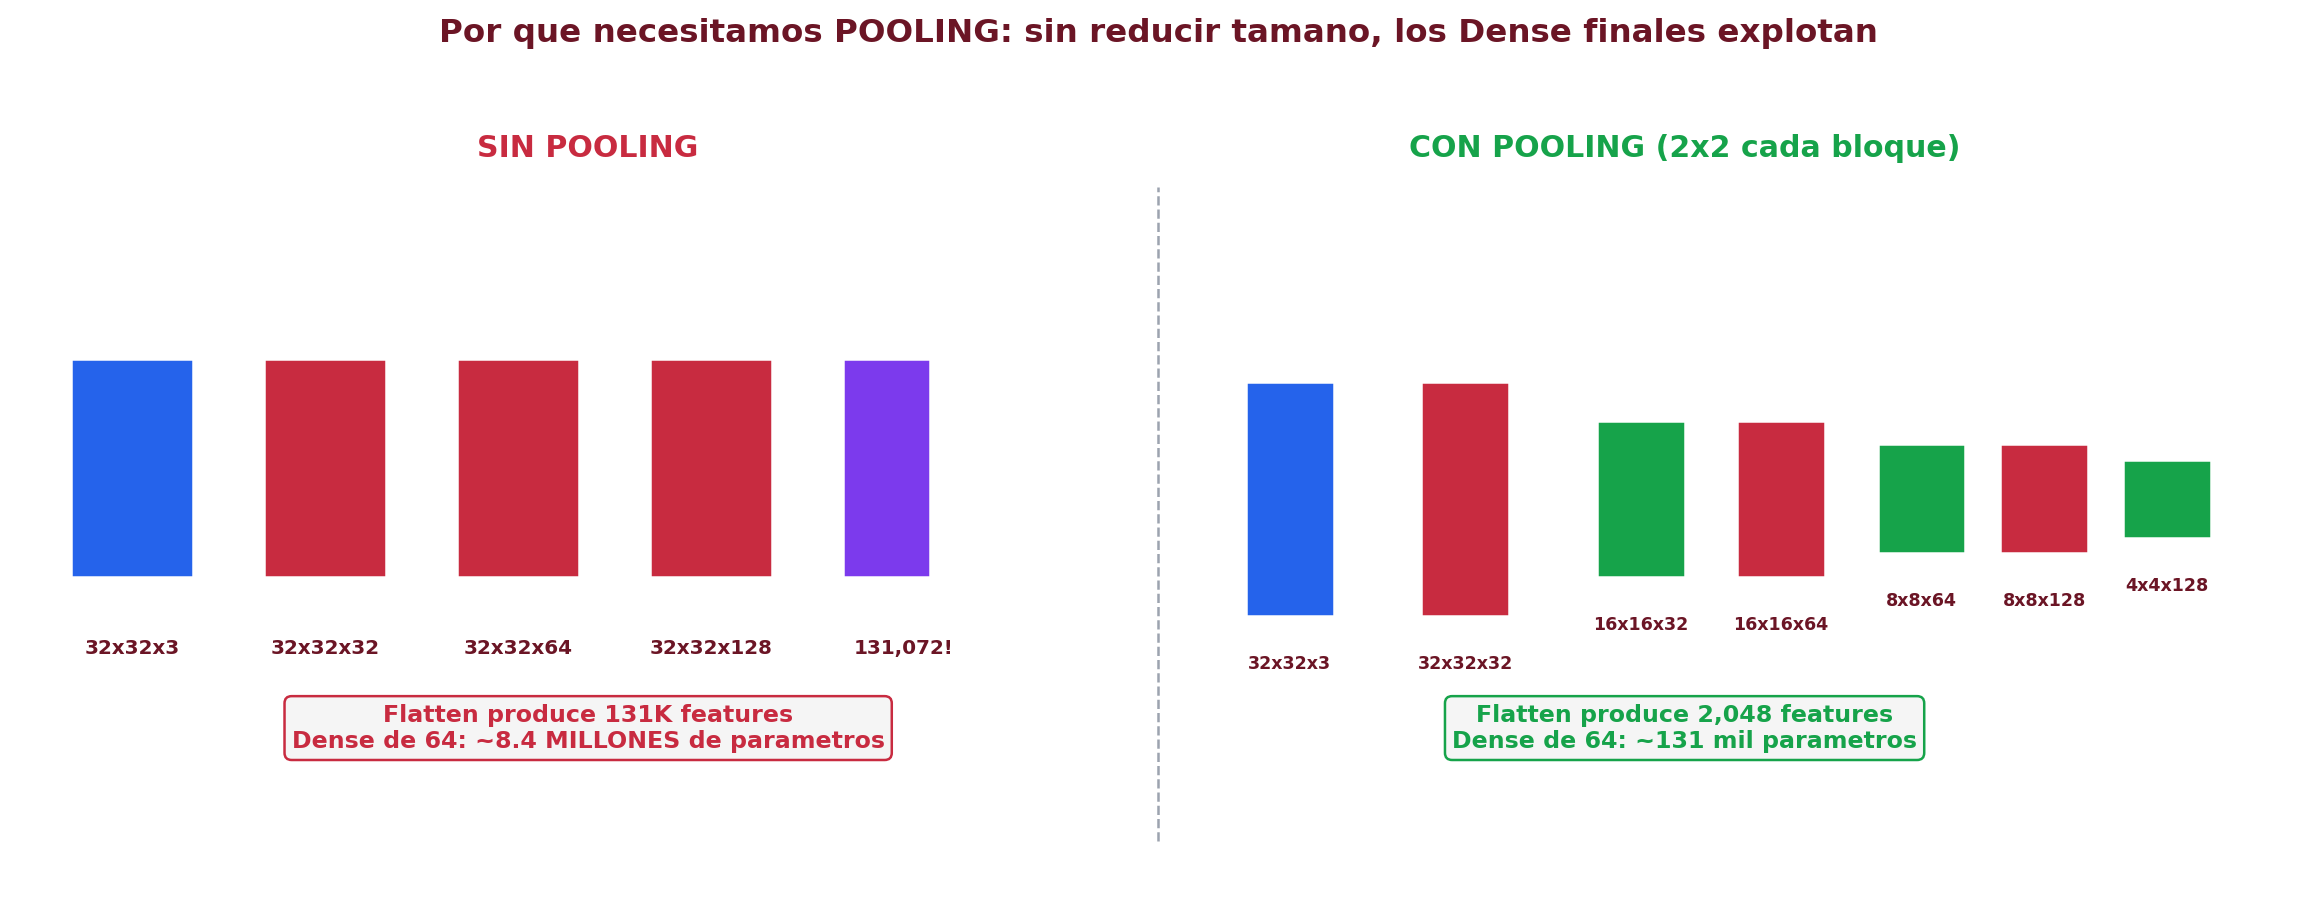
\includegraphics[width=0.95\textwidth]{fig_por_que_pool.png}
  \end{center}

  \vspace{2pt}
  {\scriptsize\color{textMuted}
    \faLightbulb\hspace{4pt} Pooling resuelve el problema reduciendo
    a la mitad cada dimensi\'on. La informaci\'on importante se conserva
    (m\'as canales), el tama\~no se reduce.}
\end{frame}

\begin{frame}[shrink]{?`Qu\'e Hace MaxPooling Exactamente?}
  \vspace{4pt}
  {\footnotesize\color{arcaDark}\bfseries
    Toma el \textbf{m\'aximo} de cada bloque 2$\times$2. La salida es
    la mitad de ancho y mitad de alto.}

  \vspace{8pt}
  \begin{center}
    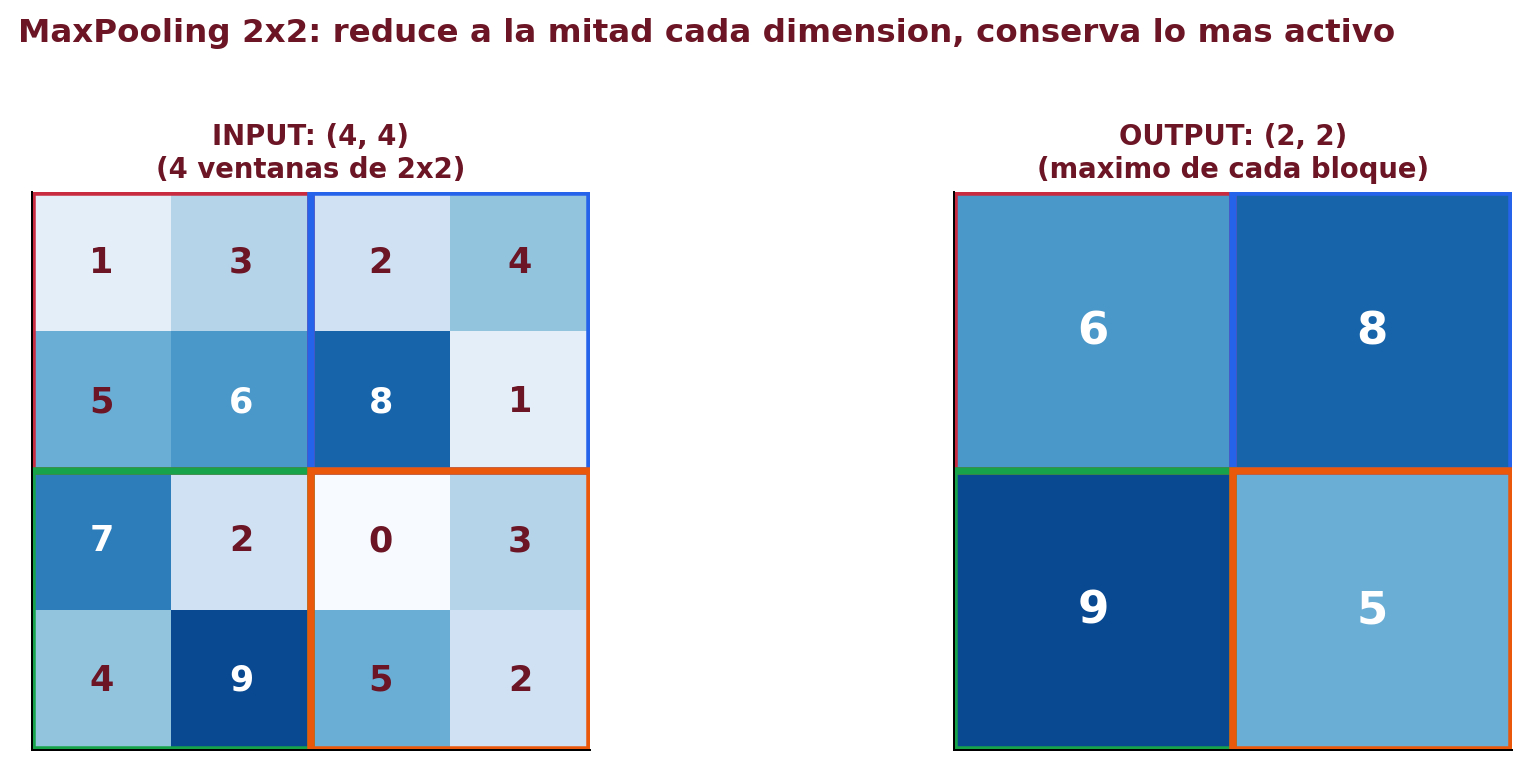
\includegraphics[width=0.78\textwidth]{fig_pooling.png}
  \end{center}

  \vspace{4pt}
  {\scriptsize
  \begin{itemize}\setlength{\itemsep}{2pt}
    \item[{\color{arcaRed}\scriptsize\faArrowRight}]
      \textbf{No tiene par\'ametros entrenables.} Es una operaci\'on
      fija (igual que \texttt{flatten}).
    \item[{\color{arcaRed}\scriptsize\faArrowRight}]
      Conserva la activaci\'on m\'as fuerte de cada zona ---
      ``donde el filtro hizo m\'as match''.
  \end{itemize}
  }
\end{frame}

\begin{frame}[shrink]{Etapa 1: Repetir el Bloque (Conv $\to$ Pool) Varias Veces}
  \vspace{6pt}
  {\footnotesize\color{arcaDark}\bfseries
    Una sola capa Conv2D detecta patrones simples (bordes). Apilando
    varias, las capas profundas combinan los patrones simples en
    \textbf{conceptos cada vez m\'as abstractos}.}

  \vspace{14pt}
  {\footnotesize
  \begin{itemize}\setlength{\itemsep}{6pt}
    \item[{\color{arcaRed}\scriptsize\faArrowRight}]
      \textbf{Bloque 1:} bordes y manchas.
    \item[{\color{arcaRed}\scriptsize\faArrowRight}]
      \textbf{Bloque 2:} esquinas, texturas, partes peque\~nas.
    \item[{\color{arcaRed}\scriptsize\faArrowRight}]
      \textbf{Bloque 3:} partes (orejas, ojos, ruedas).
    \item[{\color{codeGreen}\scriptsize\faArrowRight}]
      Esto es lo que se llama \textbf{representaci\'on jer\'arquica}.
      Es la idea m\'as importante del deep learning.
  \end{itemize}
  }
\end{frame}

\begin{frame}{Etapa 2: \texttt{Flatten} --- ?`Y Por Qu\'e?}
  \vspace{4pt}
  {\footnotesize\color{arcaDark}\bfseries
    Despu\'es de los bloques convolucionales tenemos un \textbf{tensor
    3D} (alto, ancho, canales). Pero las capas \texttt{Dense} solo
    saben procesar \textbf{vectores 1D}. Hay que convertir el formato.}

  \vspace{6pt}
  \begin{center}
    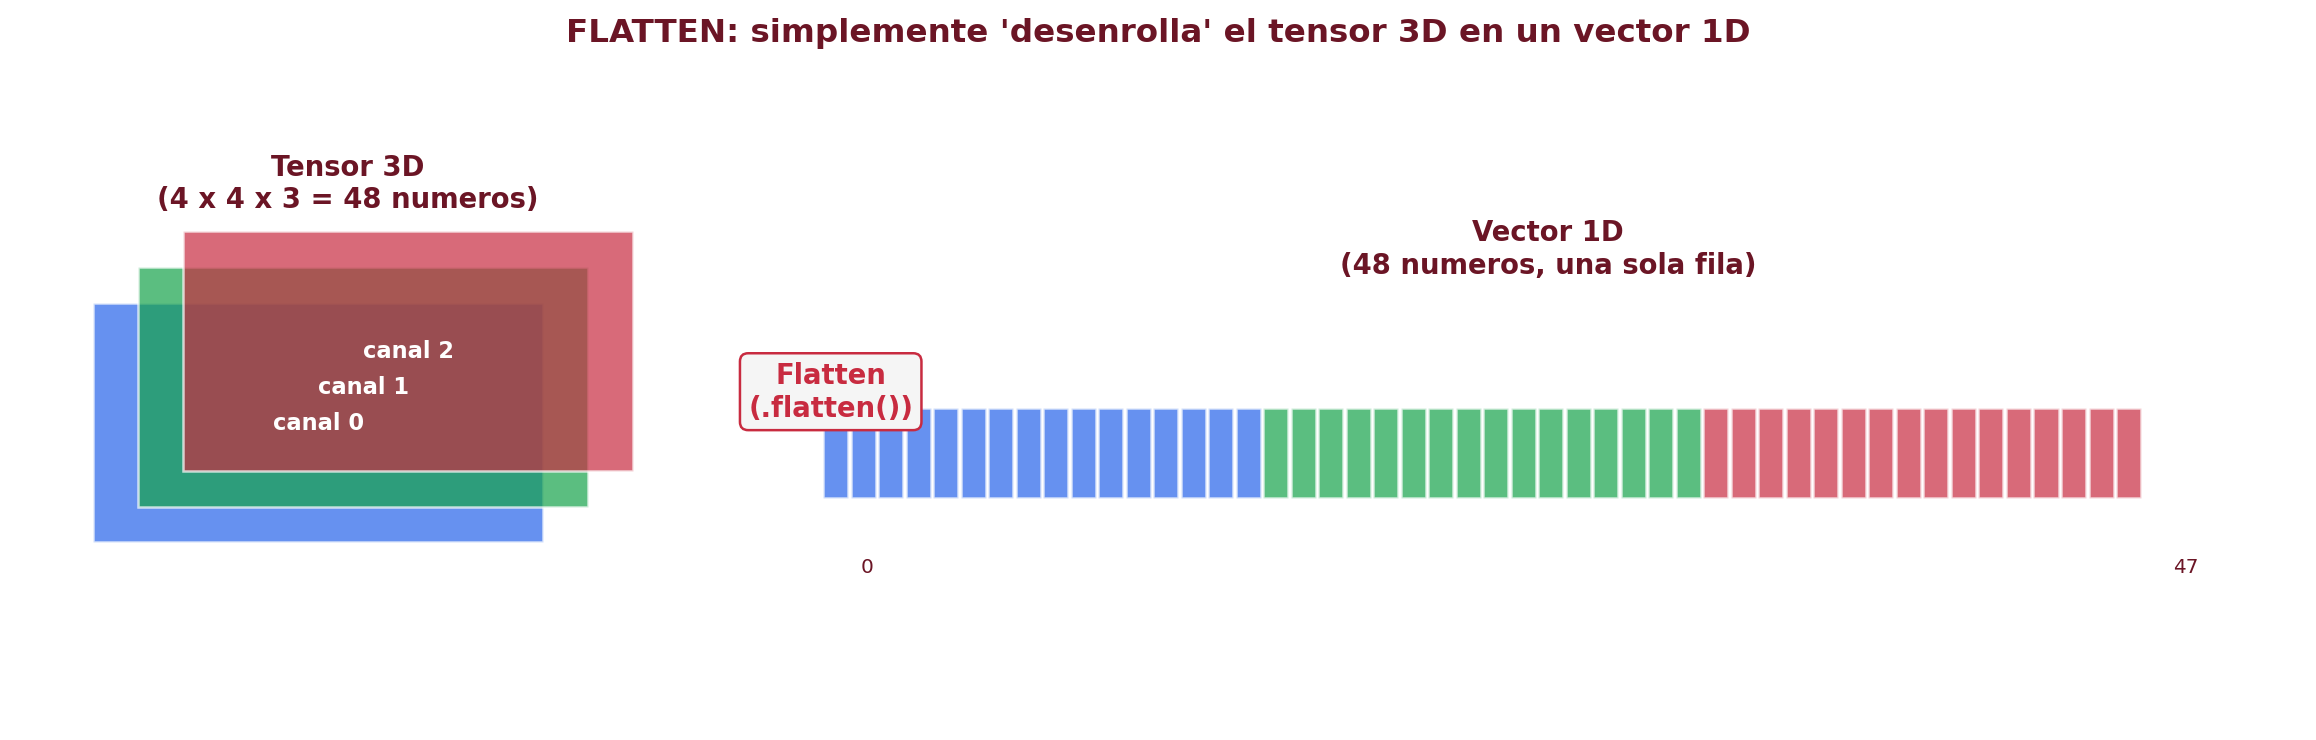
\includegraphics[width=0.95\textwidth]{fig_flatten.png}
  \end{center}

  \vspace{2pt}
  {\scriptsize\color{textMuted}
    \faLightbulb\hspace{4pt} \texttt{Flatten} simplemente \emph{desenrolla}
    el tensor en un vector. \textbf{Sin par\'ametros, sin c\'alculo} ---
    es solo cambiar la forma del array.}
\end{frame}

\begin{frame}{Etapa 3: \texttt{Dense} --- ?`Para Qu\'e Termina con un MLP?}
  \vspace{6pt}
  {\footnotesize\color{arcaDark}\bfseries
    Los bloques convolucionales \textbf{extraen} caracter\'isticas.
    Pero todav\'ia hay que tomar una \textbf{decisi\'on}:
    ``?`gato o perro?''. Esa decisi\'on la toma un MLP cl\'asico.}

  \vspace{14pt}
  {\footnotesize
  \begin{itemize}\setlength{\itemsep}{6pt}
    \item[{\color{arcaRed}\scriptsize\faArrowRight}]
      \texttt{Dense(64, activation="relu")}: una capa oculta
      (combina las caracter\'isticas extra\'idas).
    \item[{\color{arcaRed}\scriptsize\faArrowRight}]
      \texttt{Dense(N, activation="softmax")}: la \textbf{capa de
      salida} con $N$ neuronas (1 por clase).
    \item[{\color{codeGreen}\scriptsize\faArrowRight}]
      Esto es exactamente el MLP que vimos en la clase 23.
      \textbf{La CNN reusa lo que ya saben}: solo le agrega bloques
      convolucionales \emph{antes}.
  \end{itemize}
  }
\end{frame}

\begin{frame}[shrink]{Recapitulemos: Todas las Capas en una Tabla}
  \vspace{6pt}
  {\footnotesize
  \begin{tabular}{@{}p{2.4cm} p{4.0cm} p{2.5cm} p{3.5cm}@{}}
    \toprule
    \textbf{Capa} & \textbf{Qu\'e hace} & \textbf{Etapa} & \textbf{Par\'ametros} \\
    \midrule
    \rowcolor{arcaGray}
    \texttt{Conv2D}
    & Aplica filtros aprendidos.
    & Extracci\'on
    & S\'i (los filtros). \\
    \texttt{MaxPool2D}
    & Reduce a la mitad.
    & Extracci\'on
    & No (operaci\'on fija). \\
    \rowcolor{arcaGray}
    \texttt{Flatten}
    & Tensor 3D a vector 1D.
    & Aplanar
    & No (cambia forma). \\
    \texttt{Dense}
    & Capa MLP cl\'asica.
    & Clasificar
    & S\'i (pesos). \\
    \bottomrule
  \end{tabular}
  }

  \vspace{14pt}
  \begin{tcolorbox}[colback=arcaGray, colframe=arcaRed, boxrule=0.5pt,
    arc=2pt, left=6pt, right=6pt, top=4pt, bottom=4pt]
    {\scriptsize\color{arcaDark}
    \faKey\hspace{4pt}\textbf{Receta:} \texttt{(Conv $\to$ Pool)} repetido
    2--4 veces, luego \texttt{Flatten}, luego 1--2 \texttt{Dense}.}
  \end{tcolorbox}
\end{frame}

\begin{frame}[shrink]{La Arquitectura Completa Visualizada}
  \vspace{4pt}
  \begin{center}
    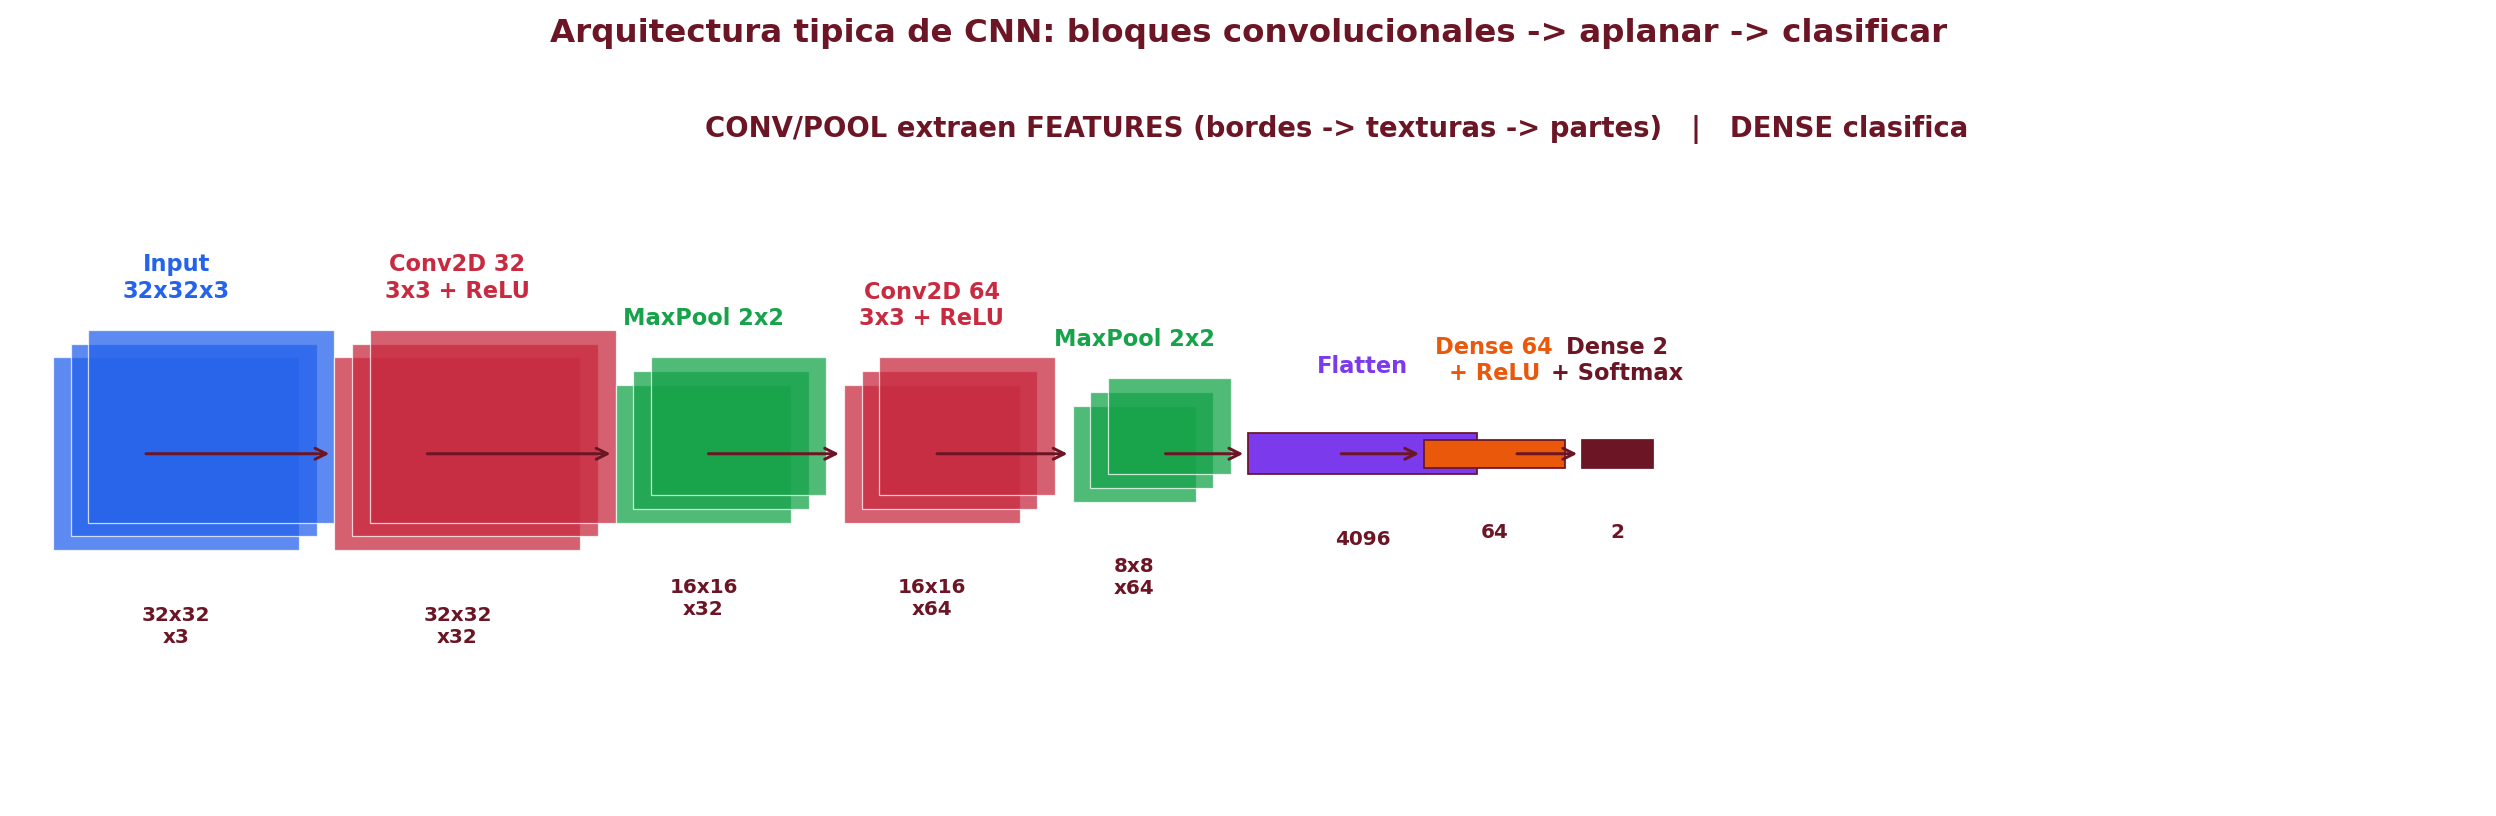
\includegraphics[width=0.97\textwidth]{fig_cnn_arquitectura.png}
  \end{center}

  \vspace{4pt}
  {\scriptsize\color{textMuted}
    \faLightbulb\hspace{4pt} Cada bloque convolucional \emph{dobla
    los filtros} y \emph{reduce a la mitad la resoluci\'on}.
    El n\'umero total de ``informaci\'on'' por imagen se mantiene
    aproximadamente constante.}
\end{frame}

\begin{frame}{C\'omo Leer \texttt{model.summary()}}
  \vspace{6pt}
  {\scriptsize
  \begin{tabular}{@{}llrr@{}}
    \toprule
    \textbf{Layer} & \textbf{Output Shape} & \textbf{\# params} & \textbf{C\'alculo} \\
    \midrule
    Conv2D 32 (3$\times$3)   & (None, 28, 28, 32)  &      320 & $32 \cdot (3 \cdot 3 \cdot 1 + 1)$ \\
    MaxPool 2$\times$2       & (None, 14, 14, 32)  &        0 & --- \\
    Conv2D 64 (3$\times$3)   & (None, 14, 14, 64)  &   18\,496 & $64 \cdot (3 \cdot 3 \cdot 32 + 1)$ \\
    MaxPool 2$\times$2       & (None, 7, 7, 64)    &        0 & --- \\
    Flatten                  & (None, 3\,136)         &        0 & --- \\
    Dense 64                 & (None, 64)          &  200\,768 & $64 \cdot (3136 + 1)$ \\
    Dense 10 (softmax)       & (None, 10)          &      650 & $10 \cdot (64 + 1)$ \\
    \midrule
    \multicolumn{2}{r}{\textbf{Total}} & \textbf{220\,234} & \\
    \bottomrule
  \end{tabular}
  }

  \vspace{12pt}
  {\scriptsize\color{textMuted}
    \faLightbulb\hspace{4pt} \textbf{Nota:} la primera Conv2D solo
    tiene \textbf{320 par\'ametros} (vs $\sim$100\,000 en un MLP
    equivalente). Eso es \emph{parameter sharing} en acci\'on.}
\end{frame}

% =============================================================================
%  BLOQUE 5: DISENAR TU CNN (CRITERIOS)
% =============================================================================
\sectionframe{Dise\~nar Tu CNN}{Cu\'antos bloques, cu\'antos filtros, qu\'e elegir}

\begin{frame}[shrink]{?`Cu\'antos Bloques Conv-Pool?}
  \vspace{4pt}
  {\footnotesize\color{arcaDark}\bfseries
    \textbf{Regla:} apilar bloques hasta que el mapa final sea
    \textbf{4$\times$4 a 8$\times$8 pixeles}. Cada MaxPool divide entre 2.}

  \vspace{14pt}
  {\footnotesize
  \begin{tabular}{@{}l c c@{}}
    \toprule
    \textbf{Imagen de entrada} & \textbf{Pools necesarios} & \textbf{Bloques recomendados} \\
    \midrule
    32$\times$32 (CIFAR)         & 2--3 (32$\to$8 o $\to$4)       & 3 \\
    64$\times$64 (foto peque\~na) & 3--4                          & 4 \\
    96$\times$96                 & 3--4                          & 4 \\
    224$\times$224 (foto web)    & 5 (224$\to$7)                 & 5 (o transfer learning) \\
    \bottomrule
  \end{tabular}
  }

  \vspace{14pt}
  {\scriptsize\color{textMuted}
    \faLightbulb\hspace{4pt} Si el mapa final es muy peque\~no (1$\times$1),
    perdimos demasiado contexto. Si es muy grande (28$\times$28), el
    Flatten genera demasiados par\'ametros.}
\end{frame}

\begin{frame}[shrink]{?`Cu\'antos Filtros en Cada Capa?}
  \vspace{4pt}
  {\footnotesize\color{arcaDark}\bfseries
    \textbf{Patr\'on cl\'asico:} doblar el n\'umero de filtros cada vez
    que se reduce la resoluci\'on espacial.}

  \vspace{14pt}
  {\footnotesize
  \begin{tabular}{@{}l c@{}}
    \toprule
    \textbf{Tama\~no del modelo} & \textbf{Progresi\'on de filtros} \\
    \midrule
    Tiny (CIFAR, MNIST)     & 32 $\to$ 64 $\to$ 128 \\
    Mediano                & 64 $\to$ 128 $\to$ 256 \\
    Grande (VGG-style)     & 64 $\to$ 128 $\to$ 256 $\to$ 512 \\
    \bottomrule
  \end{tabular}
  }

  \vspace{14pt}
  {\footnotesize\color{arcaDark}
    \textbf{Por qu\'e doblar:} la informaci\'on por imagen se conserva.
    Si la resoluci\'on baja (16$\to$8 = 1/4 de pixeles), doblar canales
    (32$\to$64) compensa. Las capas profundas detectan conceptos m\'as
    abstractos $\Rightarrow$ necesitan m\'as ``vocabulario'' (m\'as filtros).}
\end{frame}

\begin{frame}[shrink]{Tabla de Decisiones para una CNN}
  \vspace{4pt}
  \begin{center}
    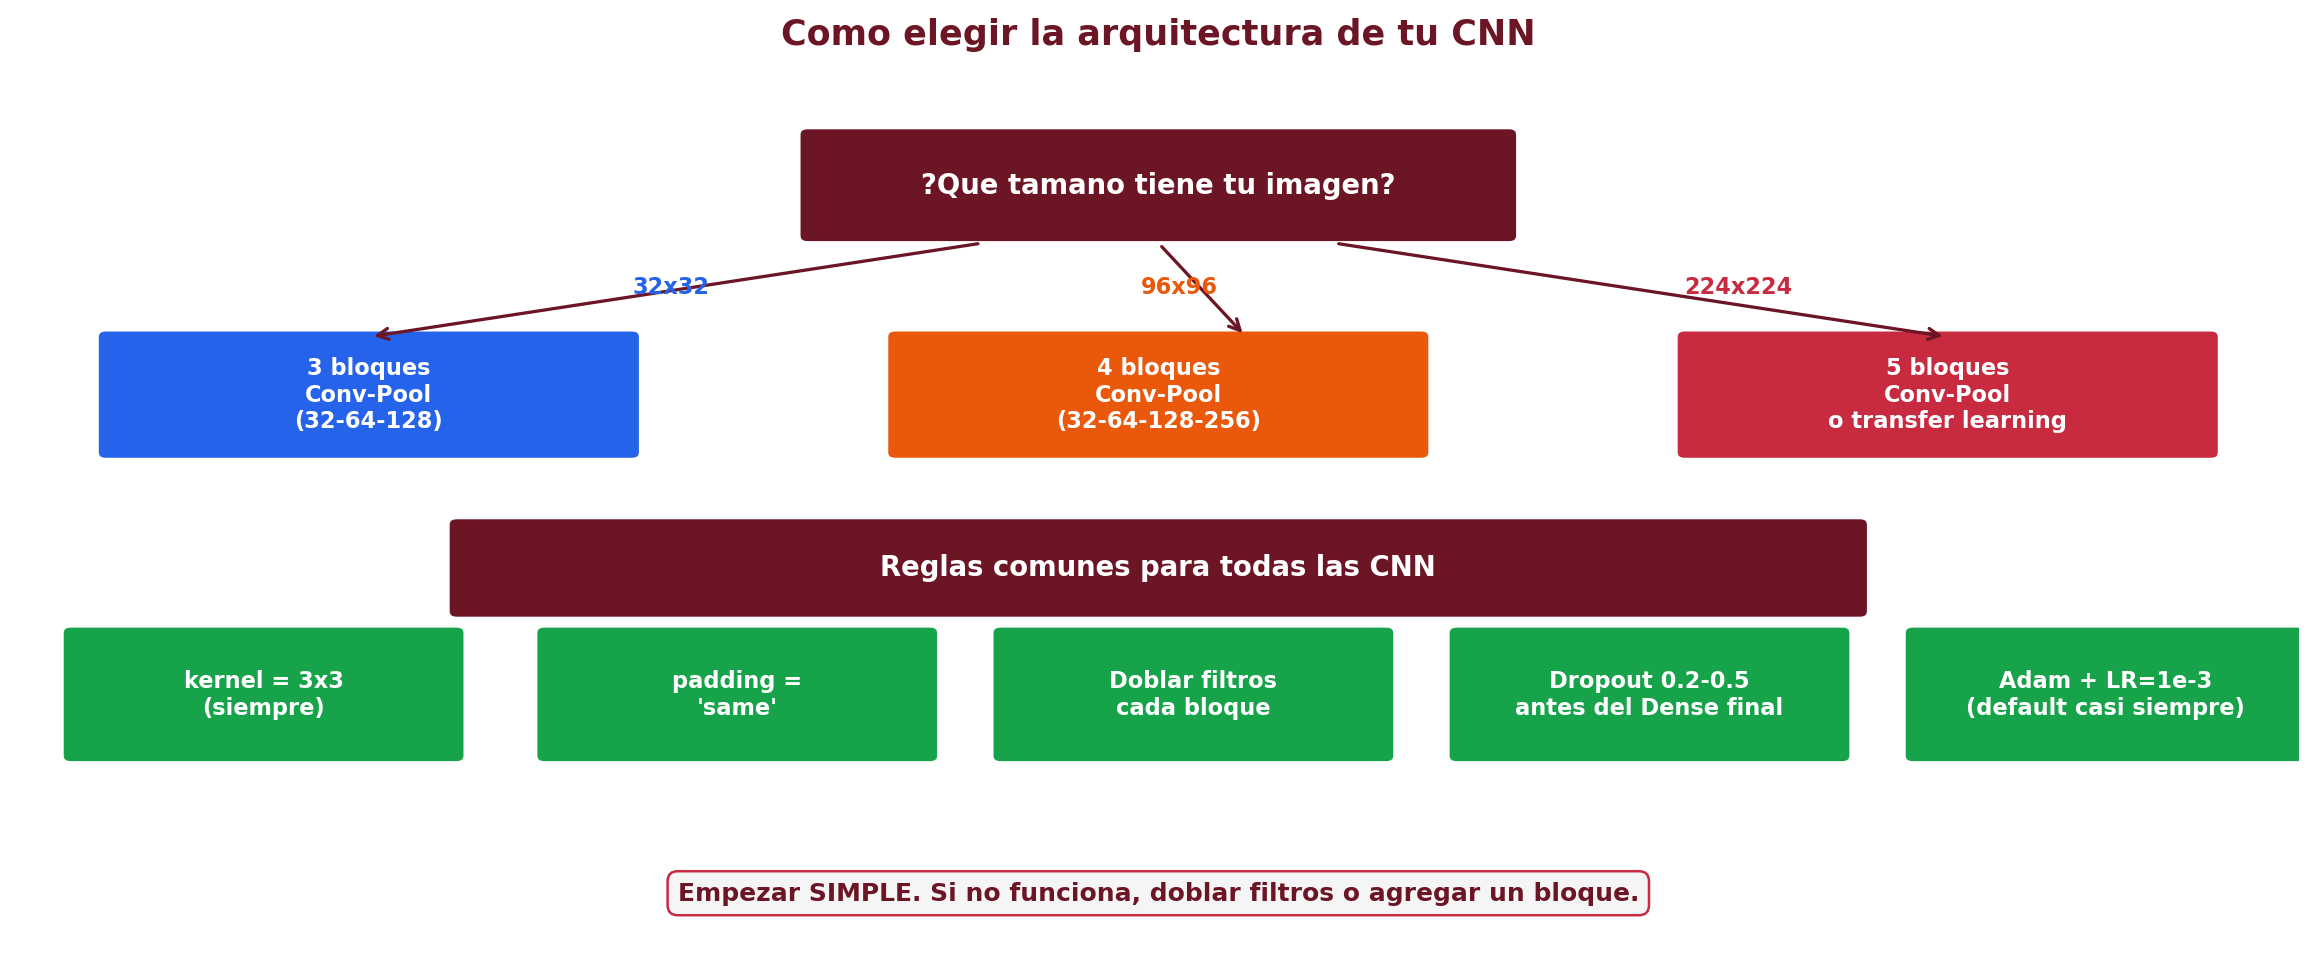
\includegraphics[width=0.95\textwidth]{fig_cnn_diseno.png}
  \end{center}

  \vspace{4pt}
  {\scriptsize\color{textMuted}
    \faLightbulb\hspace{4pt} \textbf{Empezar simple, complicar si no funciona.}
    Una CNN con 3 bloques 32-64-128 + Flatten + Dense alcanza para casi
    todo dataset peque\~no.}
\end{frame}

\begin{frame}[shrink]{Indicadores de Que Algo No Va Bien}
  \vspace{6pt}
  {\footnotesize
  \begin{tabular}{@{}p{4.5cm} p{8.0cm}@{}}
    \toprule
    \textbf{S\'intoma} & \textbf{Causa probable y soluci\'on} \\
    \midrule
    \rowcolor{arcaGray}
    Train acc alto, val acc bajo
    & \textbf{Overfitting.} Agregar Dropout (0.3--0.5),
      data augmentation, m\'as datos. \\
    Loss baja muy lento o no baja
    & Learning rate muy chico, o red muy chica. Subir LR a $10^{-3}$
      o agregar capas/filtros. \\
    \rowcolor{arcaGray}
    Loss oscila o explota
    & Learning rate muy alto, normalizar inputs (\texttt{/255}). \\
    Train y val acc parecidos pero bajos
    & \textbf{Underfitting.} Modelo muy chico, agregar bloques o filtros. \\
    \rowcolor{arcaGray}
    Acc cerca del azar
    & Verificar que las etiquetas est\'en bien, que normalizaste el input,
      que la \'ultima capa tenga las clases correctas. \\
    \bottomrule
  \end{tabular}
  }
\end{frame}

% =============================================================================
%  BLOQUE 6: KERAS Y GPU
% =============================================================================
\sectionframe{Keras y GPU}{La herramienta y por qu\'e necesitamos hardware especial}

\begin{frame}[shrink]{?`Qu\'e Es Keras?}
  \vspace{4pt}
  {\footnotesize\color{arcaDark}\bfseries
    Keras es una \textbf{API de alto nivel} para construir redes.
    No hace los c\'alculos: pide ayuda a un \emph{backend}
    (TensorFlow, JAX, PyTorch).}

  \vspace{14pt}
  \begin{center}
  \begin{tikzpicture}[
    layer/.style={rectangle, rounded corners=4pt, minimum width=11cm,
                  minimum height=0.95cm, align=center, text width=10.5cm,
                  font=\small\bfseries\color{white}, inner sep=4pt},
  ]
    \node[layer, fill=arcaDark]                  (l1) {TU C\'ODIGO (Python)\\
      {\scriptsize\mdseries\ttfamily model = Sequential([Conv2D, MaxPool, Dense])}};
    \node[layer, fill=arcaRed, below=8pt of l1]  (l2) {KERAS\\
      {\scriptsize\mdseries API de alto nivel: capas, compile, fit, evaluate}};
    \node[layer, fill=codeBlue, below=8pt of l2] (l3) {BACKEND: TensorFlow / JAX / PyTorch\\
      {\scriptsize\mdseries quien hace los gradientes y la GPU}};
    \node[layer, fill=textDark, below=8pt of l3] (l4) {GPU / CPU / TPU\\
      {\scriptsize\mdseries quien ejecuta las matrices}};

    \draw[->, line width=1.5pt, arcaDark] (l1.south) -- (l2.north);
    \draw[->, line width=1.5pt, arcaDark] (l2.south) -- (l3.north);
    \draw[->, line width=1.5pt, arcaDark] (l3.south) -- (l4.north);
  \end{tikzpicture}
  \end{center}

  \vspace{4pt}
  {\scriptsize\color{textMuted}
    \faLightbulb\hspace{4pt} Origen 2015, Fran\c{c}ois Chollet (Google).
    Hoy es la API oficial de TensorFlow (\texttt{tf.keras}).}
\end{frame}

\begin{frame}[shrink]{?`Por Qu\'e Keras y No PyTorch Puro?}
  \vspace{6pt}
  {\footnotesize
  \begin{tabular}{@{}p{6.0cm} p{6.5cm}@{}}
    \toprule
    \textbf{\color{codeBlue}Keras} & \textbf{\color{codePurple}PyTorch puro} \\
    \midrule
    \texttt{model.fit(X, y)} igual que \texttt{LogisticRegression}.
    & Loop manual: \texttt{loss.backward()}, \texttt{optimizer.step()}\ldots \\
    \rowcolor{arcaGray}
    Bater\'ias incluidas (m\'etricas, callbacks, EarlyStopping).
    & M\'as control, m\'as l\'ineas para lo b\'asico. \\
    Excelente para \textbf{prototipar} y \textbf{ense\~nar}.
    & Estandar en \textbf{investigaci\'on} y modelos custom complejos. \\
    \bottomrule
  \end{tabular}
  }

  \vspace{14pt}
  \begin{tcolorbox}[colback=codeGreen!8, colframe=codeGreen, boxrule=0.5pt,
    arc=2pt, left=6pt, right=6pt, top=4pt, bottom=4pt]
    {\scriptsize\color{arcaDark}
    \faKey\hspace{4pt}\textbf{Pedag\'ogicamente:} aprenden Keras hoy,
    transfieren a PyTorch ma\~nana. Los conceptos son los mismos
    (capas, optimizer, loss, gradient).}
  \end{tcolorbox}
\end{frame}

\begin{frame}[fragile,shrink]{La API: Una Sola Mirada}
  \vspace{-4pt}
  \begin{pyblock}
from tensorflow import keras
from tensorflow.keras import layers, Sequential

model = Sequential([
    layers.Conv2D(32, 3, activation="relu", input_shape=(32,32,3)),
    layers.MaxPooling2D(),
    layers.Conv2D(64, 3, activation="relu"),
    layers.MaxPooling2D(),
    layers.Flatten(),
    layers.Dense(64, activation="relu"),
    layers.Dense(2, activation="softmax"),
])

model.compile("adam", "sparse_categorical_crossentropy", ["accuracy"])
model.fit(X_train, y_train, epochs=10, validation_split=0.2)
  \end{pyblock}
\end{frame}

\begin{frame}[shrink]{?`Por Qu\'e las CNN Necesitan GPU?}
  \vspace{4pt}
  {\footnotesize\color{arcaDark}\bfseries
    Una CNN hace \emph{millones} de multiplicaciones por imagen.
    Multiplicar por 50\,000 im\'agenes y 50 epochs = trillones de
    operaciones.}

  \vspace{8pt}
  \begin{center}
    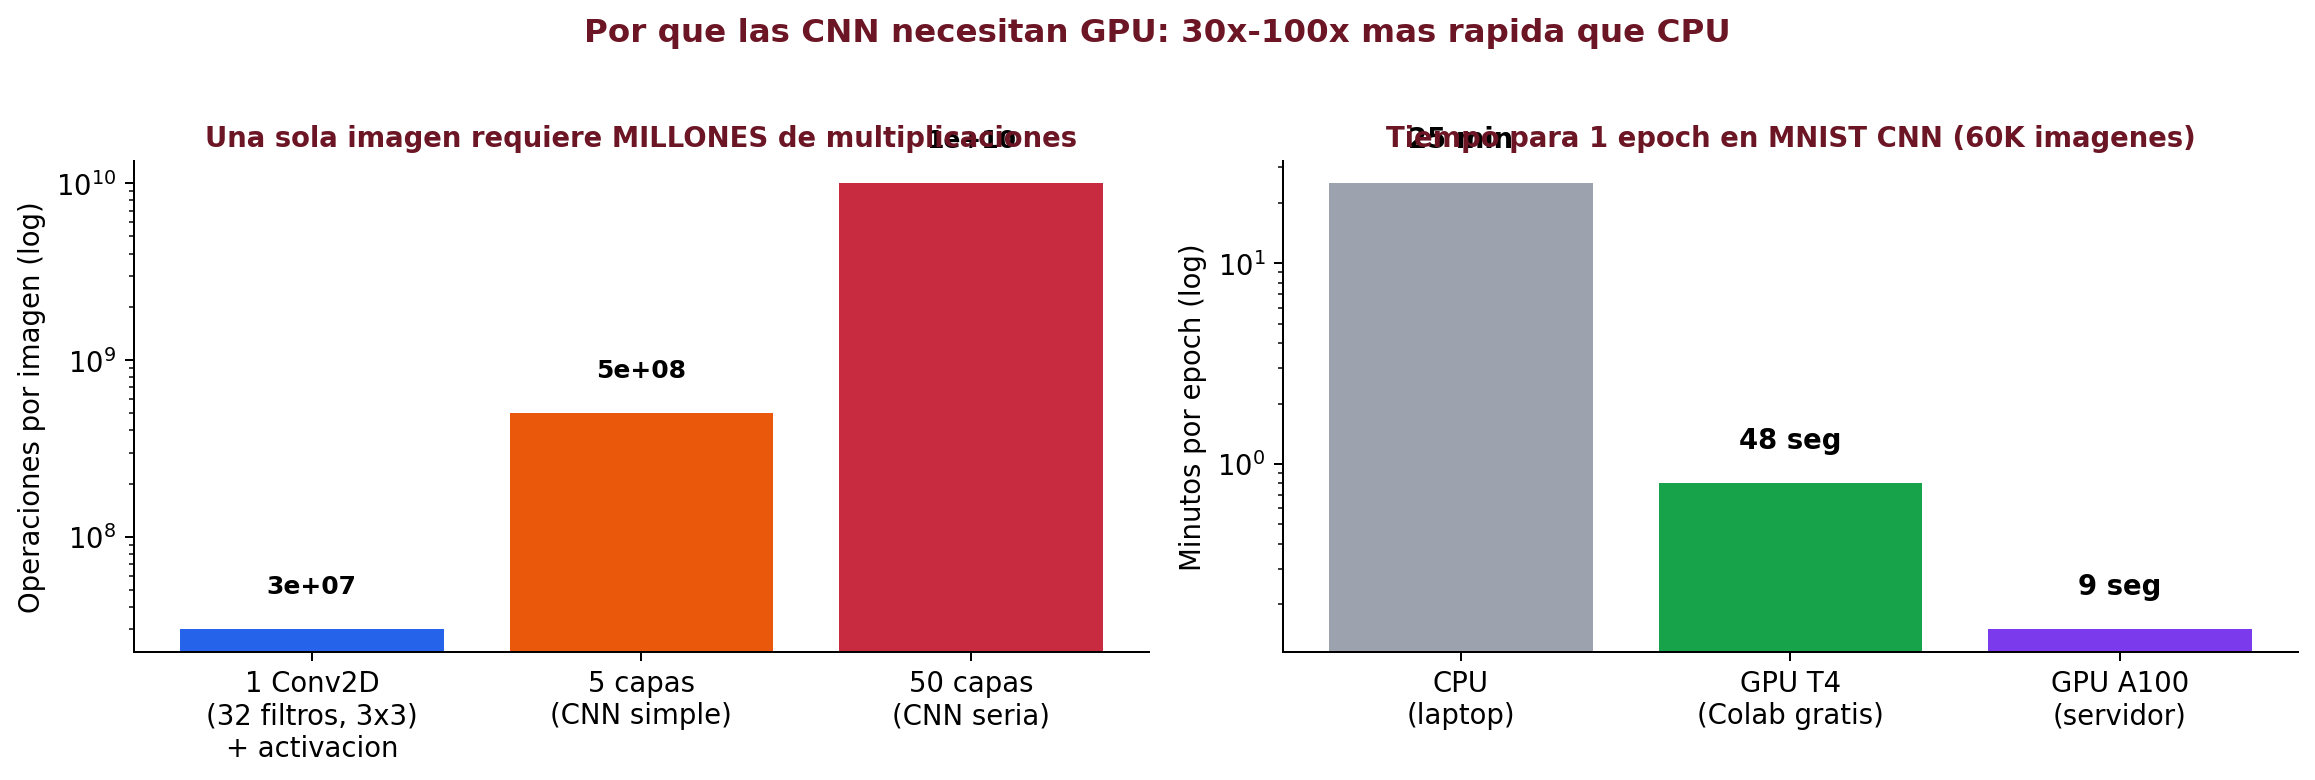
\includegraphics[width=0.95\textwidth]{fig_gpu_vs_cpu.png}
  \end{center}

  \vspace{4pt}
  {\scriptsize\color{textMuted}
    \faLightbulb\hspace{4pt} Las GPUs hacen \textbf{miles de
    multiplicaciones en paralelo} (lo que las CPUs hacen una a una).
    Por eso son 30--100$\times$ m\'as r\'apidas para CNN.}
\end{frame}

\begin{frame}[shrink]{C\'omo Activar GPU en Google Colab}
  \vspace{8pt}
  {\footnotesize\color{arcaDark}\bfseries
    Colab da GPU gratis (T4) con un click. Hay que activarla \emph{antes}
    de ejecutar c\'odigo:}

  \vspace{14pt}
  {\footnotesize
  \begin{enumerate}\setlength{\itemsep}{6pt}
    \item[{\color{arcaRed}\bfseries 1.}]
      Men\'u: \texttt{Runtime $\to$ Change runtime type}.
    \item[{\color{arcaRed}\bfseries 2.}]
      \textbf{Hardware accelerator:} elegir \texttt{T4 GPU}.
    \item[{\color{arcaRed}\bfseries 3.}]
      Save. El runtime se reinicia.
    \item[{\color{codeGreen}\bfseries 4.}]
      Verificar:
      \texttt{tf.config.list\_physical\_devices("GPU")}
      debe devolver una lista no vac\'ia.
  \end{enumerate}
  }

  \vspace{14pt}
  \begin{tcolorbox}[colback=codeOrange!8, colframe=codeOrange, boxrule=0.5pt,
    arc=2pt, left=6pt, right=6pt, top=4pt, bottom=4pt]
    {\scriptsize\color{arcaDark}
    \faExclamationTriangle\hspace{4pt}\textbf{Cuidado:} la GPU se
    desconecta tras 1--2 horas inactivas. Guardar pesos con
    \texttt{model.save("modelo.keras")} para no perder el entrenamiento.}
  \end{tcolorbox}
\end{frame}

% =============================================================================
%  BLOQUE 7: CNN EN ACCION
% =============================================================================
\sectionframe{CNN en Acci\'on}{De MNIST a cats vs dogs}

\begin{frame}[fragile,shrink]{C\'odigo: CNN M\'inima en MNIST}
  \vspace{-4pt}
  \begin{pyblock}
(X_tr, y_tr), (X_te, y_te) = keras.datasets.mnist.load_data()
X_tr, X_te = X_tr[..., None]/255.0, X_te[..., None]/255.0

cnn = Sequential([
    layers.Conv2D(32, 3, activation="relu", input_shape=(28,28,1)),
    layers.MaxPooling2D(),
    layers.Conv2D(64, 3, activation="relu"),
    layers.MaxPooling2D(),
    layers.Flatten(),
    layers.Dense(64, activation="relu"),
    layers.Dense(10, activation="softmax"),
])
cnn.compile("adam", "sparse_categorical_crossentropy", ["accuracy"])
cnn.fit(X_tr, y_tr, epochs=5, validation_split=0.1)
  \end{pyblock}
\end{frame}

\begin{frame}[shrink]{Resultados: La Pared Se Vuelve Camino}
  \vspace{4pt}
  \begin{center}
    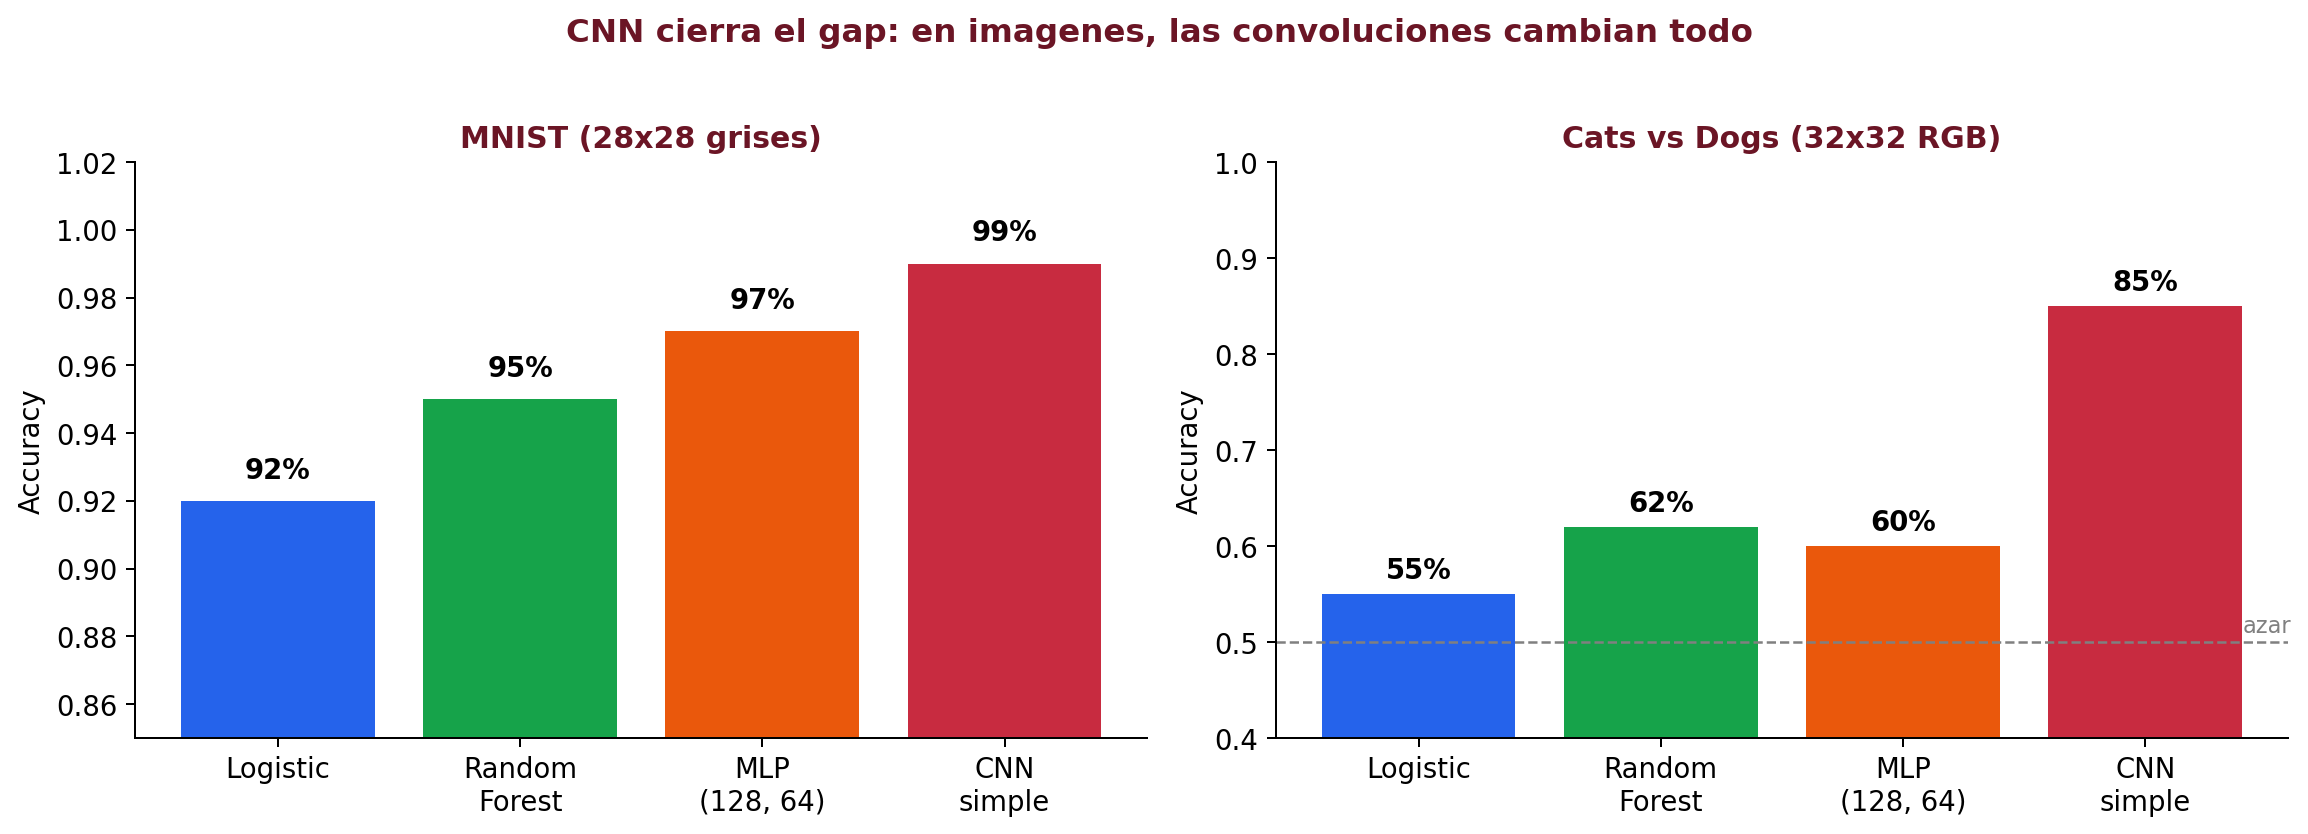
\includegraphics[width=0.95\textwidth]{fig_resultados_cnn.png}
  \end{center}

  \vspace{4pt}
  {\scriptsize\color{textMuted}
    \faLightbulb\hspace{4pt} \textbf{MNIST:} CNN llega a $\sim$99\%
    (humano $\approx$ 99.7\%). \textbf{Cats vs Dogs:} con la \emph{misma}
    data de la clase 22, la CNN salta de $\sim$60\% a $\sim$85\%.
    La diferencia es \emph{toda} arquitectural.}
\end{frame}

\begin{frame}[shrink]{Data Augmentation: M\'as Datos Sin Recolectar}
  \vspace{4pt}
  {\footnotesize\color{arcaDark}\bfseries
    Truco esencial cuando hay pocos datos: generar variaciones
    (rotar, voltear, brillo) durante el entrenamiento.}

  \vspace{6pt}
  \begin{center}
    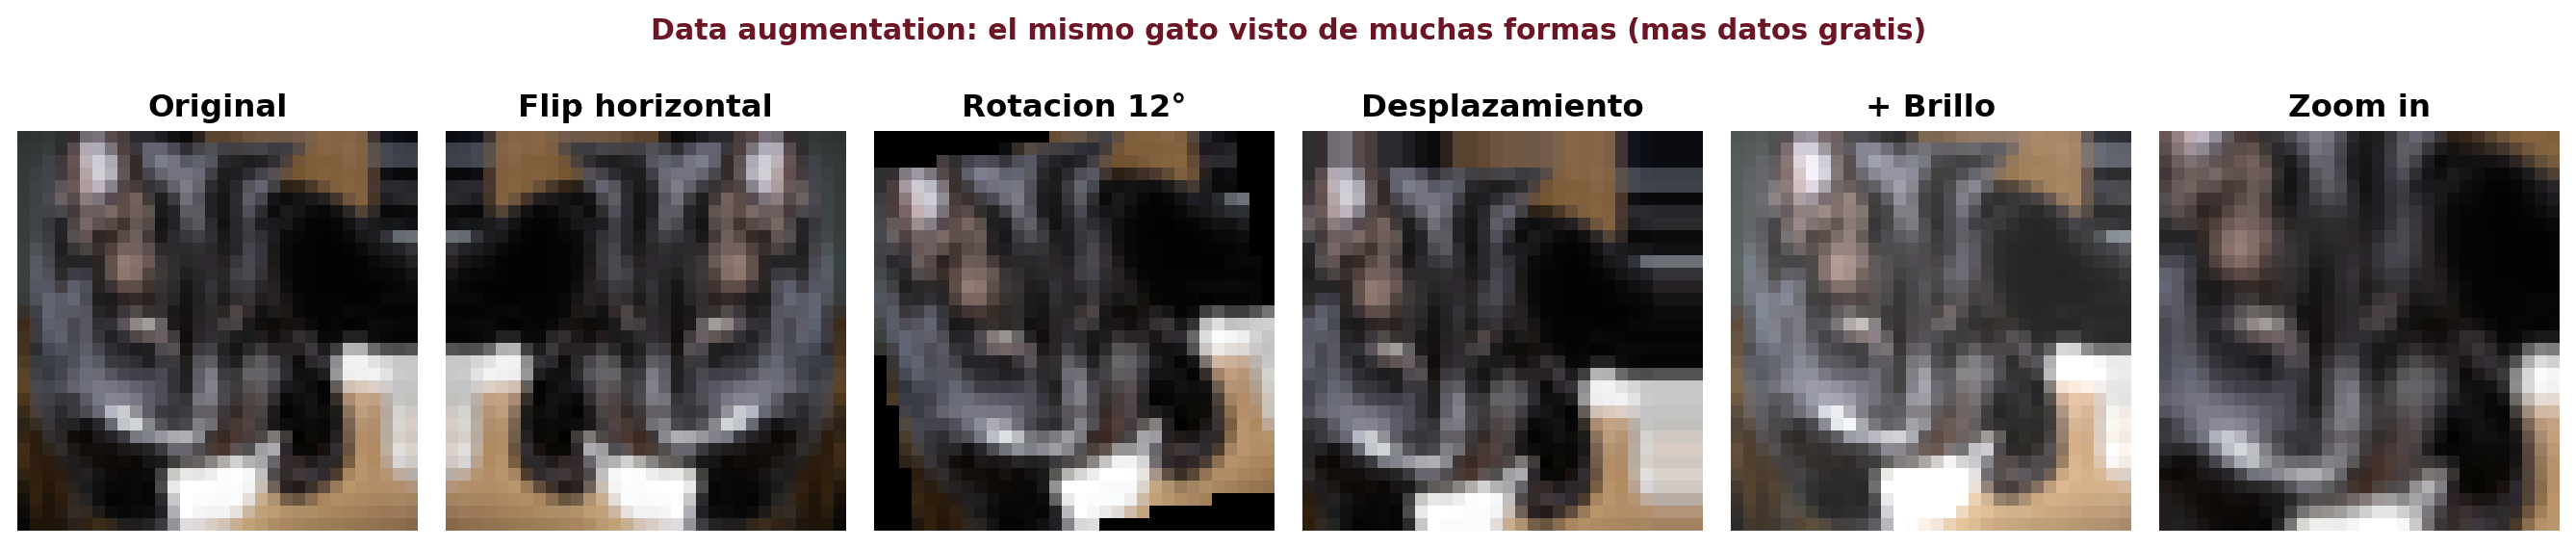
\includegraphics[width=0.97\textwidth]{fig_data_aug.png}
  \end{center}

  \vspace{4pt}
  {\scriptsize\color{textMuted}
    \faLightbulb\hspace{4pt} En Keras se hace agregando capas
    \texttt{RandomFlip}, \texttt{RandomRotation}, \texttt{RandomZoom}
    al inicio del modelo. En cats vs dogs sube otros 5--7 puntos.}
\end{frame}

% =============================================================================
%  BLOQUE 8: TRANSFER LEARNING
% =============================================================================
\sectionframe{Transfer Learning}{Reusar lo que otra red ya aprendi\'o}

\begin{frame}[shrink]{La Idea: Misma Red, Nueva Tarea}
  \vspace{4pt}
  {\footnotesize\color{arcaDark}\bfseries
    Si una CNN aprendi\'o a distinguir gatos y perros, sus filtros
    aprendieron a detectar \textbf{bordes, texturas y formas}. Eso
    sirve para distinguir \emph{cualquier} cosa visual.}

  \vspace{6pt}
  \begin{center}
    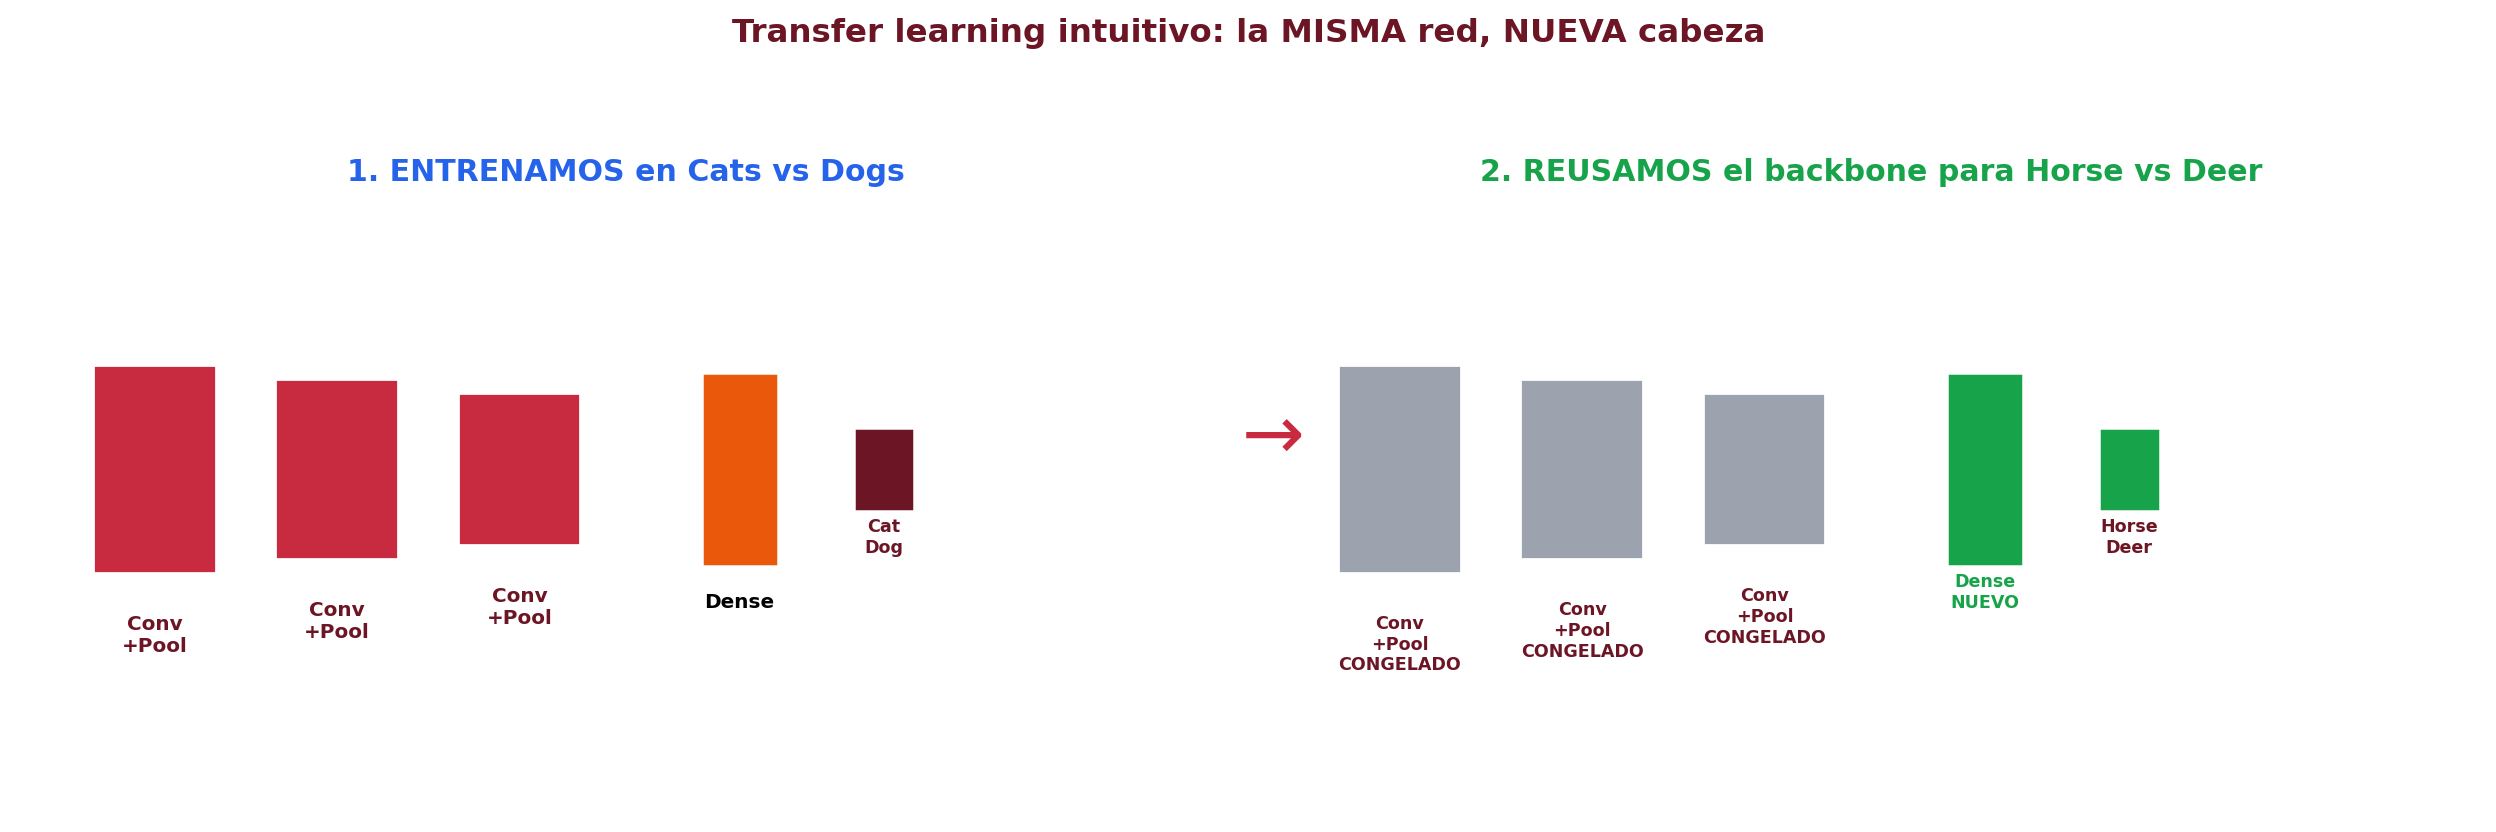
\includegraphics[width=0.95\textwidth]{fig_transfer_misma_red.png}
  \end{center}

  \vspace{4pt}
  {\scriptsize\color{textMuted}
    \faLightbulb\hspace{4pt} Para una nueva tarea: \emph{congelamos}
    los bloques convolucionales (no se reentrenan) y solo entrenamos
    una nueva cabeza Dense. Mucho menos datos y mucho menos c\'omputo.}
\end{frame}

\begin{frame}[shrink]{?`Por Qu\'e Funciona?}
  \vspace{8pt}
  {\footnotesize\color{arcaDark}\bfseries
    Las primeras capas convolucionales aprenden conceptos que son
    \textbf{los mismos en cualquier tarea de visi\'on}:}

  \vspace{14pt}
  {\footnotesize
  \begin{itemize}\setlength{\itemsep}{6pt}
    \item[{\color{arcaRed}\scriptsize\faArrowRight}]
      \textbf{Capas tempranas:} bordes, manchas, gradientes simples.
    \item[{\color{arcaRed}\scriptsize\faArrowRight}]
      \textbf{Capas medias:} texturas, esquinas, patrones repetitivos.
    \item[{\color{arcaRed}\scriptsize\faArrowRight}]
      \textbf{Capas tard\'ias:} partes (orejas, ojos, ruedas) y luego objetos.
    \item[{\color{codeGreen}\scriptsize\faArrowRight}]
      Solo las \emph{\'ultimas} capas son espec\'ificas de la tarea.
      Reusamos las primeras y reentrenamos las \'ultimas.
  \end{itemize}
  }
\end{frame}

\begin{frame}[shrink]{Modelos P\'ublicos: ?`Qu\'e Es ImageNet?}
  \vspace{4pt}
  {\footnotesize\color{arcaDark}\bfseries
    No es f\'acil entrenar una CNN buena: hace falta mucha data y
    mucha GPU. Por suerte otros ya lo hicieron --- en un dataset
    p\'ublico llamado \textbf{ImageNet}.}

  \vspace{14pt}
  \begin{center}
  \begin{tikzpicture}[
    fact/.style={rectangle, rounded corners=4pt, minimum width=2.7cm,
                 minimum height=2.6cm, align=center, text width=2.5cm,
                 inner sep=4pt, font=\scriptsize\color{white}},
  ]
    \node[fact, fill=codeBlue] (f1)
      {{\bfseries\large 1.4 millones}\\{\bfseries de im\'agenes}\\[4pt]
       Etiquetadas a mano por humanos};
    \node[fact, fill=codeOrange, right=6pt of f1] (f2)
      {{\bfseries\large 1\,000}\\{\bfseries categor\'ias}\\[4pt]
       Perros, autos, frutas, herramientas, animales\ldots};
    \node[fact, fill=codePurple, right=6pt of f2] (f3)
      {{\bfseries\large 224$\times$224}\\{\bfseries resoluci\'on}\\[4pt]
       Fotos reales del mundo (no MNIST)};
    \node[fact, fill=codeGreen, right=6pt of f3] (f4)
      {{\bfseries\large 2010--2017}\\{\bfseries Concurso}\\[4pt]
       Donde nacieron VGG, ResNet, Inception\ldots};
  \end{tikzpicture}
  \end{center}

  \vspace{8pt}
  {\scriptsize\color{textMuted}
    \faLightbulb\hspace{4pt} VGG16 ``vio'' 1.4M de fotos. Sus filtros
    aprendieron lo que es un \textbf{borde}, una \textbf{textura},
    un \textbf{ojo}. Sirven para casi cualquier problema de visi\'on.}
\end{frame}

\begin{frame}[shrink]{VGG16: La M\'as F\'acil de Leer}
  \vspace{4pt}
  {\footnotesize\color{arcaDark}\bfseries
    \textbf{VGG16} (Oxford, 2014) es una CNN que solo apila lo que
    ya conocemos: \texttt{Conv2D 3$\times$3} + \texttt{MaxPool} +
    \texttt{Dense}. \emph{Sin bloques especiales, sin atajos}.}

  \vspace{6pt}
  \begin{center}
    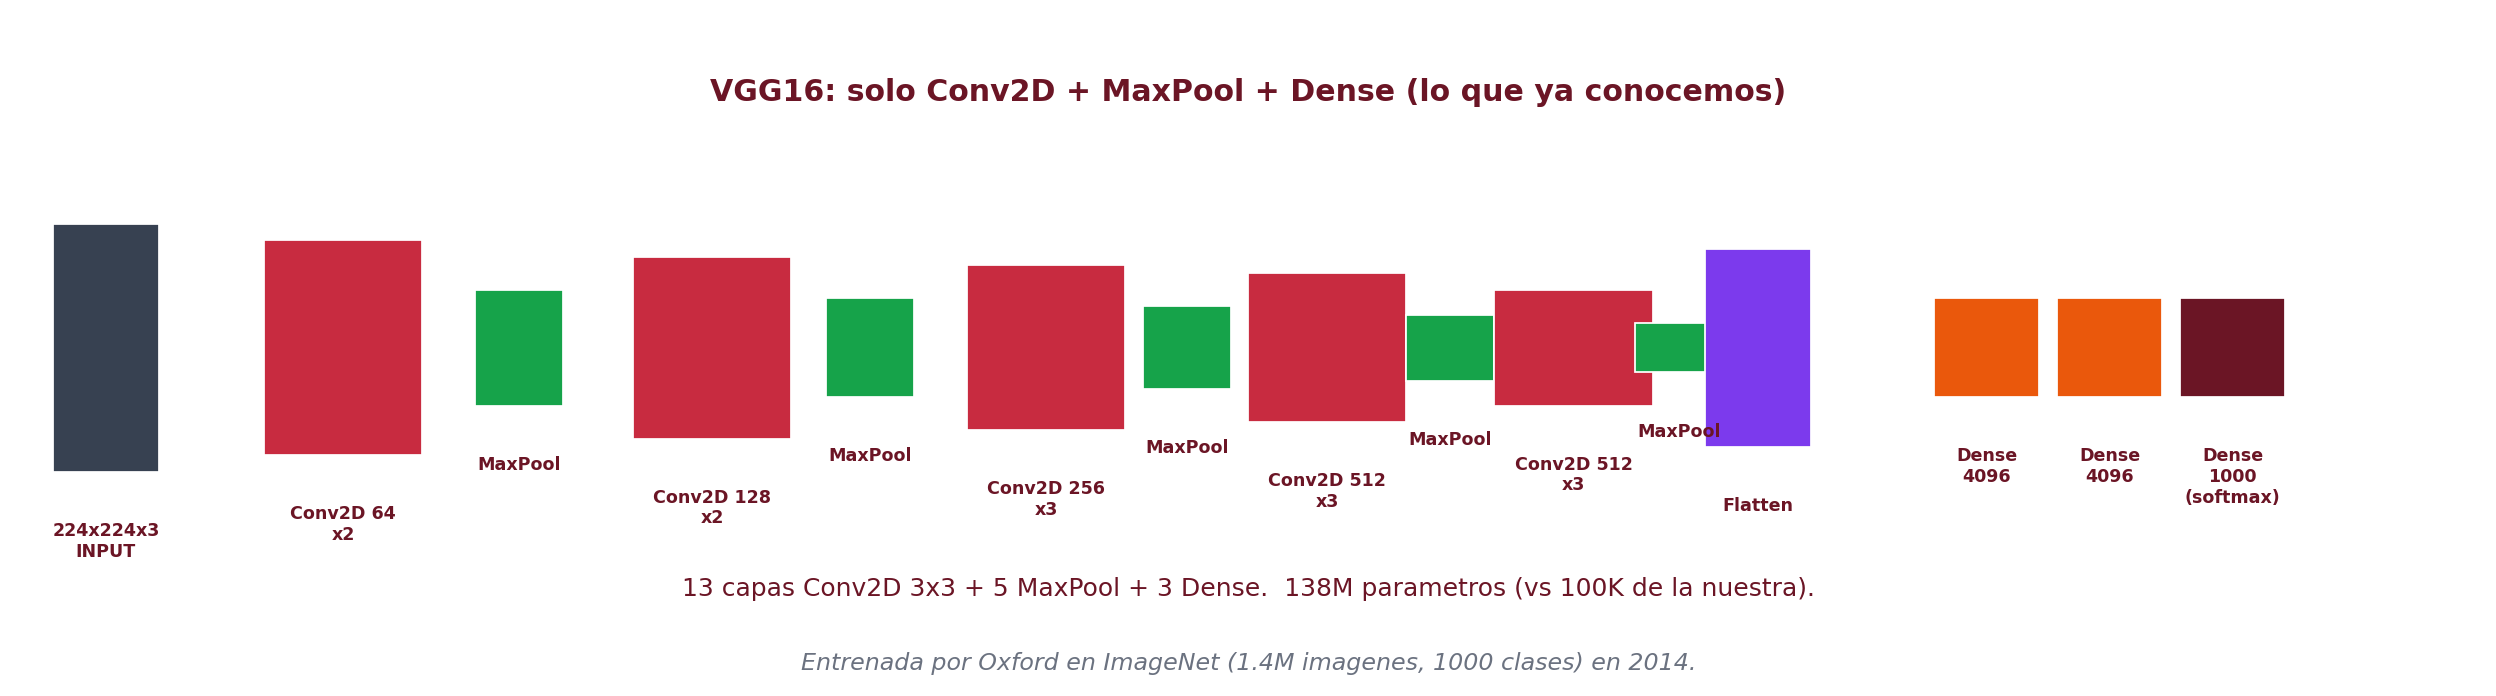
\includegraphics[width=0.97\textwidth]{fig_vgg16.png}
  \end{center}

  \vspace{2pt}
  {\scriptsize\color{textMuted}
    \faLightbulb\hspace{4pt} Esa simplicidad la hace
    \textbf{ideal para entender}. Existen modelos m\'as modernos
    (ResNet, EfficientNet) que son m\'as rapidos pero con bloques
    avanzados que veremos despu\'es.}
\end{frame}

\begin{frame}[shrink]{?`C\'omo Compara con Nuestra CNN?}
  \vspace{14pt}
  \begin{center}
  {\footnotesize
  \begin{tabular}{@{}>{\raggedright\arraybackslash}p{4cm}
                   >{\centering\arraybackslash}p{4cm}
                   >{\centering\arraybackslash}p{4cm}@{}}
    \toprule
    & \textbf{\color{arcaRed}Nuestra CNN}
    & \textbf{\color{codeGreen}VGG16} \\
    & {\scriptsize la que entrenamos hoy}
    & {\scriptsize la que reusamos} \\
    \midrule
    \rowcolor{arcaGray}
    Datos de entrenamiento
    & 4\,000 imagenes (cats vs dogs)
    & \textbf{1.4 millones} (ImageNet) \\
    Par\'ametros
    & $\sim$120 mil
    & \textbf{138 millones} \\
    \rowcolor{arcaGray}
    Capas convolucionales
    & 3 (Conv-Pool $\times$3)
    & \textbf{13} (5 bloques) \\
    Tiempo de entrenamiento (con GPU)
    & $\sim$2 minutos
    & \textbf{$\sim$3 semanas} (en 2014) \\
    \bottomrule
  \end{tabular}
  }
  \end{center}

  \vspace{12pt}
  \begin{tcolorbox}[colback=arcaRed!8, colframe=arcaRed, boxrule=0.5pt,
    arc=2pt, left=6pt, right=6pt, top=4pt, bottom=4pt]
    {\scriptsize\color{arcaDark}
    \faExclamationTriangle\hspace{4pt}\textbf{Imposible que nuestra CNN
    compita desde cero.} Por eso reusamos los pesos de VGG16: aunque
    nuestra tarea es distinta, \emph{los patrones visuales b\'asicos
    son los mismos}.}
  \end{tcolorbox}
\end{frame}

\begin{frame}[fragile,shrink]{Transfer Learning con VGG16 en C\'odigo}
  \vspace{-4pt}
  \begin{pyblock}
from tensorflow.keras.applications import VGG16

# 1. Cargar VGG16 SIN su cabeza, con pesos de ImageNet
base = VGG16(input_shape=(96,96,3), include_top=False, weights="imagenet")
base.trainable = False                 # congelar capas conv

# 2. Backbone congelado + cabeza nueva
modelo = Sequential([
    base,
    layers.Flatten(),
    layers.Dense(64, activation="relu"),
    layers.Dense(2, activation="softmax"),
])

# 3. Solo entrena el cabezal (pocos pesos, pocas epochs)
modelo.compile("adam", "sparse_categorical_crossentropy", ["accuracy"])
modelo.fit(X_train, y_train, epochs=5, validation_split=0.1)
  \end{pyblock}
\end{frame}

% =============================================================================
%  BLOQUE 9: LIMITACIONES
% =============================================================================
\sectionframe{Limitaciones}{Cu\'ando NO entrenar una CNN desde cero}

\begin{frame}[shrink]{Cuatro Costos Reales de las CNN}
  \vspace{6pt}
  {\footnotesize
  \begin{tabular}{@{}p{2.6cm} p{10.0cm}@{}}
    \toprule
    \textbf{Costo} & \textbf{C\'omo se manifiesta} \\
    \midrule
    \rowcolor{arcaGray}
    \textbf{Datos}
    & Una CNN seria pide decenas de miles de im\'agenes etiquetadas.
      Si tienen 500, una CNN desde cero \emph{no funciona}. \\
    \textbf{C\'omputo}
    & GPU pr\'acticamente obligatoria. Sin ella, entrenar dataset grande
      toma horas o d\'ias. \\
    \rowcolor{arcaGray}
    \textbf{Hiperpar\'ametros}
    & Filtros, profundidad, learning rate, batch, dropout\ldots
      Mucho m\'as tuning que sklearn. \\
    \textbf{Interpretabilidad}
    & Dif\'icil decir ``por qu\'e'' la CNN predijo gato. T\'ecnicas
      como Grad-CAM ayudan, pero no como ``feature importance'' de RF. \\
    \bottomrule
  \end{tabular}
  }

  \vspace{14pt}
  \begin{tcolorbox}[colback=codeOrange!8, colframe=codeOrange, boxrule=0.5pt,
    arc=2pt, left=6pt, right=6pt, top=4pt, bottom=4pt]
    {\scriptsize\color{arcaDark}
    \faExclamationTriangle\hspace{4pt}\textbf{Antes de entrenar desde cero:}
    pregunten si pueden usar transfer learning. La respuesta casi siempre
    es s\'i.}
  \end{tcolorbox}
\end{frame}

\begin{frame}[shrink]{?`Cu\'ando Usar (y NO Usar) una CNN?}
  \vspace{4pt}
  \begin{center}
    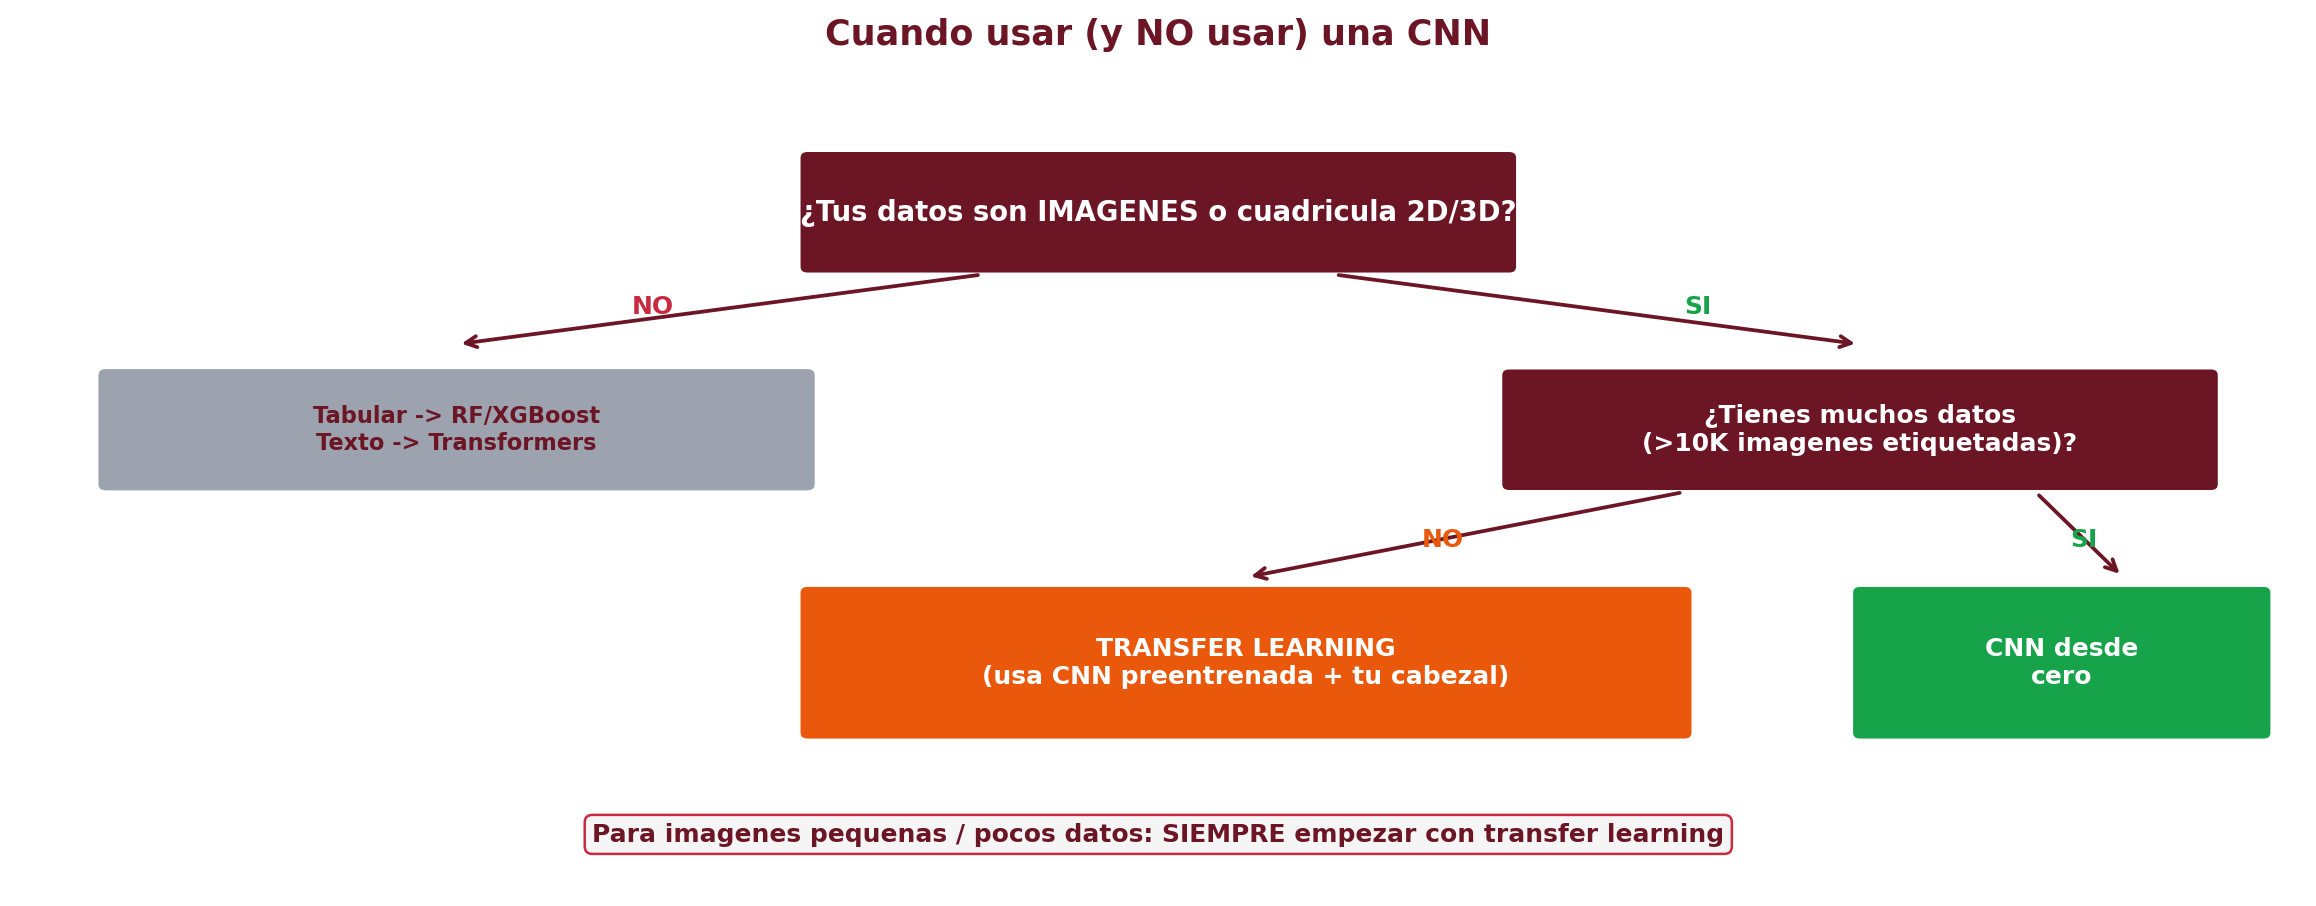
\includegraphics[width=0.92\textwidth]{fig_cuando_cnn.png}
  \end{center}

  \vspace{4pt}
  {\scriptsize
  \begin{itemize}\setlength{\itemsep}{2pt}
    \item[{\color{codeGreen}\scriptsize\faCheck}]
      \textbf{S\'i} CNN: im\'agenes, espectrogramas de audio,
      datos en cuadr\'icula 2D/3D.
    \item[{\color{arcaRed}\scriptsize\faTimes}]
      \textbf{No} CNN para tabular (RF/XGBoost), texto (Transformers),
      series temporales no espaciales.
  \end{itemize}
  }
\end{frame}

\begin{frame}[shrink]{Una Mirada al Futuro: Vision Transformers}
  \vspace{6pt}
  {\footnotesize\color{arcaDark}\bfseries
    Desde 2020 las \textbf{Vision Transformers (ViT)} compiten y
    a veces superan a las CNN. Importante saberlo --- pero
    nuestra base sigue siendo CNN.}

  \vspace{14pt}
  {\footnotesize
  \begin{itemize}\setlength{\itemsep}{6pt}
    \item[{\color{arcaRed}\scriptsize\faArrowRight}]
      \textbf{ViT} divide la imagen en parches 16$\times$16 y los trata
      como ``palabras'', con el mismo mecanismo que GPT.
    \item[{\color{arcaRed}\scriptsize\faArrowRight}]
      Modelos modernos (CLIP, DINOv2, Stable Diffusion) son a base de
      transformers / h\'ibridos.
    \item[{\color{codeGreen}\scriptsize\faArrowRight}]
      \textbf{Pero las CNN siguen siendo el caballo de batalla} cuando
      hay poca data, pocos recursos o restricciones de latencia
      (m\'oviles, IoT, l\'ineas de producci\'on).
  \end{itemize}
  }
\end{frame}

% =============================================================================
%  BLOQUE 10: EJERCICIO FINAL --- CONSTRUIR TU PROPIO DATASET
% =============================================================================
\sectionframe{Ejercicio Final}{Construye tu propio dataset y entrena un clasificador}

\begin{frame}[shrink]{Tu Turno: Resolver un Problema Real}
  \vspace{6pt}
  {\footnotesize\color{arcaDark}\bfseries
    Hasta ahora usamos datasets que alguien m\'as recolect\'o. Ahora
    \textbf{ustedes} construyen el dataset \textbf{y} el clasificador.
    Para un problema que tenga sentido para Arca o para su \'area.}

  \vspace{14pt}
  {\footnotesize\color{arcaDark}\bfseries Ideas de problemas binarios (eligen uno o proponen otro):}

  \vspace{6pt}
  {\footnotesize
  \begin{itemize}\setlength{\itemsep}{4pt}
    \item[{\color{arcaRed}\scriptsize\faArrowRight}]
      \textbf{Anaquel lleno vs anaquel vac\'io} ---
      \emph{caso real de retail.} Detectar autom\'aticamente cu\'ando una g\'ondola
      necesita reposici\'on.
    \item[{\color{arcaRed}\scriptsize\faArrowRight}]
      \textbf{Lata vs botella PET} --- formato de empaque (f\'acil de buscar im\'agenes).
    \item[{\color{arcaRed}\scriptsize\faArrowRight}]
      \textbf{Producto Arca vs competencia} (Coca vs Inca, etc.).
    \item[{\color{arcaRed}\scriptsize\faArrowRight}]
      \textbf{Etiqueta legible vs da\~nada} --- control de calidad.
    \item[{\color{arcaRed}\scriptsize\faArrowRight}]
      \textbf{Camion cargado vs vac\'io} --- log\'istica.
    \item[{\color{codeGreen}\scriptsize\faArrowRight}]
      \textbf{Tu propuesta:} cualquier problema relevante a tu trabajo.
  \end{itemize}
  }
\end{frame}

\begin{frame}[shrink]{Construir un Buen Dataset: 5 Reglas de Oro}
  \vspace{6pt}
  {\footnotesize
  \begin{tabular}{@{}p{3.5cm} p{9.0cm}@{}}
    \toprule
    \textbf{Regla} & \textbf{Por qu\'e importa} \\
    \midrule
    \rowcolor{arcaGray}
    \textbf{1. Balance de clases}
    & Similar n\'umero de fotos por clase. Si tienes 200 ``llenas''
      y 20 ``vac\'ias'', el modelo aprende a decir ``lleno'' siempre. \\
    \textbf{2. Diversidad}
    & Distintos \'angulos, luces, distancias, fondos. Si todas las
      ``vac\'ias'' son del mismo Oxxo, el modelo aprende el \emph{Oxxo},
      no el ``vac\'io''. \\
    \rowcolor{arcaGray}
    \textbf{3. Train/test disjuntos}
    & Nunca dejar la misma foto (ni casi-duplicados) en train y test.
      Si no, el accuracy es una mentira. \\
    \textbf{4. Etiquetado consistente}
    & Las clases deben ser inequ\'ivocas. ?`Qu\'e es ``medio lleno''?
      Definir reglas \emph{antes} de etiquetar. \\
    \rowcolor{arcaGray}
    \textbf{5. Calidad $\,>\,$ cantidad}
    & 200 fotos buenas y diversas $>$ 1\,000 fotos repetitivas.
      Mejor menos pero limpio. \\
    \bottomrule
  \end{tabular}
  }
\end{frame}

\begin{frame}[shrink]{Errores Comunes (No Caigan en Estos)}
  \vspace{6pt}
  {\footnotesize
  \begin{tabular}{@{}p{4.5cm} p{8.0cm}@{}}
    \toprule
    \textbf{Error} & \textbf{Qu\'e pasa} \\
    \midrule
    \rowcolor{arcaRed!8}
    \textbf{Sesgo de fuente}
    & Todas las ``llenas'' de Google Images, todas las ``vac\'ias'' de
      Pinterest. El modelo aprende \emph{el sitio web}, no el problema. \\
    \textbf{Resoluci\'on inconsistente}
    & Mezclar fotos 4K con fotos 100$\times$100. Resize a un tama\~no
      \'unico (96$\times$96 o 224$\times$224) ANTES de entrenar. \\
    \rowcolor{arcaRed!8}
    \textbf{Im\'agenes ambiguas}
    & ``Anaquel medio lleno'' --- ?`d\'onde va? Decidir reglas
      previamente o agregar una clase ``intermedia''. \\
    \textbf{Test set contaminado}
    & Agregar fotos del mismo evento (mismo d\'ia, misma tienda) en
      train y test. Test debe venir de \emph{otra} tienda u otro d\'ia. \\
    \rowcolor{arcaRed!8}
    \textbf{Ignorar la distribuci\'on de producci\'on}
    & Si el modelo va a usarse de noche con luz tenue, no entrenar
      solo con fotos de d\'ia. El dataset debe parecerse a la realidad
      donde ser\'a desplegado. \\
    \bottomrule
  \end{tabular}
  }
\end{frame}

\begin{frame}[shrink]{D\'onde Conseguir Im\'agenes}
  \vspace{6pt}
  {\footnotesize
  \begin{tabular}{@{}p{3.8cm} p{8.5cm}@{}}
    \toprule
    \textbf{Fuente} & \textbf{Cu\'ando usarla} \\
    \midrule
    \rowcolor{arcaGray}
    \textbf{Google Images / Bing}
    & R\'apido, mucha variedad, pero cuidado con sesgos.
      M\'as f\'acil para problemas gen\'ericos (perro, gato, lata). \\
    \textbf{Tu propio celular}
    & La mejor opci\'on para problemas espec\'ificos de tu trabajo.
      Salir a tomar fotos en distintas tiendas / l\'ineas. \\
    \rowcolor{arcaGray}
    \textbf{Webcam con Gradio}
    & Captar fotos en vivo desde el notebook. Ideal para
      datasets peque\~nos. \\
    \textbf{Datasets p\'ublicos}
    & \texttt{kaggle.com}, \texttt{huggingface.co/datasets},
      \texttt{Open Images}. Buscar el problema antes de empezar de cero. \\
    \rowcolor{arcaGray}
    \textbf{Web scraping}
    & Cuando hay un sitio espec\'ifico (catalogo de productos).
      Verificar t\'erminos de uso. \\
    \bottomrule
  \end{tabular}
  }

  \vspace{8pt}
  \begin{tcolorbox}[colback=codeGreen!8, colframe=codeGreen, boxrule=0.5pt,
    arc=2pt, left=6pt, right=6pt, top=4pt, bottom=4pt]
    {\scriptsize\color{arcaDark}
    \faKey\hspace{4pt}\textbf{Para empezar:} 50--100 fotos por clase
    desde Google Images. Si funciona, ampl\'iar con fotos propias.}
  \end{tcolorbox}
\end{frame}

\begin{frame}[shrink]{Plan de Trabajo (Para Esta Semana)}
  \vspace{6pt}
  {\footnotesize\color{arcaDark}\bfseries
    Lo construimos paso a paso en el notebook (\texttt{Clase\_24\_CNN.ipynb}).
    Entregable: link p\'ublico de Gradio + screenshot de m\'etricas.}

  \vspace{12pt}
  \begin{center}
  \begin{tikzpicture}[
    pstep/.style={rectangle, rounded corners=4pt, minimum width=2.4cm,
                 minimum height=1.7cm, align=center, text width=2.2cm,
                 inner sep=4pt, font=\scriptsize\color{white}\bfseries},
  ]
    \node[pstep, fill=codeBlue]   (s1)
      {1. ELEGIR\\problema\\\scriptsize\mdseries y 2--3 clases};
    \node[pstep, fill=codeOrange, right=4pt of s1] (s2)
      {2. RECOLECTAR\\50--100 por clase\\\scriptsize\mdseries diverso};
    \node[pstep, fill=codePurple, right=4pt of s2] (s3)
      {3. ETIQUETAR\\y limpiar\\\scriptsize\mdseries reglas claras};
    \node[pstep, fill=arcaRed, right=4pt of s3]   (s4)
      {4. ENTRENAR\\transfer learning\\\scriptsize\mdseries VGG16 + cabeza};
    \node[pstep, fill=codeGreen, right=4pt of s4] (s5)
      {5. EVALUAR\\confusion matrix\\\scriptsize\mdseries no solo accuracy};
    \node[pstep, fill=arcaDark, right=4pt of s5]  (s6)
      {6. DESPLEGAR\\Gradio app\\\scriptsize\mdseries link p\'ublico};

    \draw[->, line width=1pt, arcaDark] (s1) -- (s2);
    \draw[->, line width=1pt, arcaDark] (s2) -- (s3);
    \draw[->, line width=1pt, arcaDark] (s3) -- (s4);
    \draw[->, line width=1pt, arcaDark] (s4) -- (s5);
    \draw[->, line width=1pt, arcaDark] (s5) -- (s6);
  \end{tikzpicture}
  \end{center}

  \vspace{8pt}
  {\scriptsize\color{textMuted}
    \faLightbulb\hspace{4pt} \textbf{Pr\'oxima clase:} cada quien presenta
    su modelo en 3 minutos: qu\'e clasifica, c\'omo arm\'o el dataset,
    qu\'e accuracy logr\'o, d\'onde fall\'o.}
\end{frame}

% =============================================================================
%  CIERRE
% =============================================================================
\sectionframe{Cierre}{Lo que aprendimos hoy}

\begin{frame}[shrink]{Resumen}
  \vspace{4pt}
  \begin{columns}[T]
    \begin{column}{0.48\textwidth}
      {\footnotesize\bfseries\color{arcaDark} El problema:}
      \vspace{4pt}

      {\scriptsize
      MLP no es invariante, explota en par\'ametros, ignora estructura
      espacial. Resultado: $\sim$60\% en cats vs dogs.

      \vspace{8pt}
      \textbf{La idea (CNN):}

      \vspace{4pt}
      Filtros 3$\times$3 compartidos que recorren la imagen. Pocos
      par\'ametros, autom\'aticamente invariantes a posici\'on,
      capturan estructura local.
      }
    \end{column}
    \begin{column}{0.48\textwidth}
      {\footnotesize\bfseries\color{arcaDark} La caja de herramientas:}
      \vspace{4pt}

      {\scriptsize
      \texttt{Conv2D}, \texttt{MaxPool}, \texttt{Flatten}, \texttt{Dense}.
      Misma API \texttt{.fit()/.predict()} que sklearn.
      Keras + TensorFlow + GPU.

      \vspace{8pt}
      \textbf{Transfer learning:}

      \vspace{4pt}
      VGG16 preentrenada + cabezal nuevo. Resuelve el caso de
      poca data (la mayor\'ia de proyectos reales).
      }
    \end{column}
  \end{columns}

  \vspace{14pt}
  \begin{tcolorbox}[colback=codeGreen!8, colframe=codeGreen, boxrule=0.5pt,
    arc=2pt, left=6pt, right=6pt, top=4pt, bottom=4pt]
    {\scriptsize\color{arcaDark}
    \faKey\hspace{4pt}\textbf{Lo m\'as importante:} la idea de aprender
    representaciones jer\'arquicas (bordes $\to$ texturas $\to$ objetos)
    a partir de datos. Esa idea mueve toda la IA moderna.}
  \end{tcolorbox}
\end{frame}

\begin{frame}[shrink]{?`Qu\'e Viene Despu\'es?}
  \vspace{6pt}
  {\footnotesize\color{arcaDark}\bfseries
    Sigue el m\'odulo de \textbf{IA Generativa}, donde estos mismos
    bloques se usan para \emph{generar}, no solo clasificar:}

  \vspace{14pt}
  {\footnotesize
  \begin{itemize}\setlength{\itemsep}{6pt}
    \item[{\color{arcaRed}\scriptsize\faArrowRight}]
      \textbf{Autoencoders:} comprimir y reconstruir im\'agenes.
      Base de detecci\'on de anomal\'ias.
    \item[{\color{arcaRed}\scriptsize\faArrowRight}]
      \textbf{Variational AE / GANs:} generar im\'agenes nuevas
      que parecen reales.
    \item[{\color{arcaRed}\scriptsize\faArrowRight}]
      \textbf{Diffusion models:} la familia detr\'as de Midjourney y DALL-E.
    \item[{\color{codeGreen}\scriptsize\faArrowRight}]
      \textbf{LLMs multimodales} (GPT-4V, Gemini): visi\'on + lenguaje.
  \end{itemize}
  }
\end{frame}

% ── QR DE CIERRE ──────────────────────────────────────────────────────
{
\setbeamertemplate{headline}{}
\setbeamertemplate{footline}{}
\begin{frame}[plain, noframenumbering]
  \begin{tikzpicture}[remember picture, overlay]
    \fill[arcaDark] (current page.south west) rectangle (current page.north east);
  \end{tikzpicture}
  \vspace{1.0cm}
  \begin{center}
    {\color{white}\Huge\bfseries Encuesta de Cierre} \\[0.4cm]
    {\color{white!85}\Large Cu\'entanos qu\'e tal estuvo la clase}
    \vspace{1cm}

    
\includegraphics[width=4.5cm]{qr_encuesta.jpg}

    \vspace{0.6cm}
    {\color{white!80}\small Gracias por hoy}
  \end{center}
\end{frame}
}

\end{document}
